\documentclass{mimosis}
\KOMAoptions{open=any}

\usepackage{ebgaramond}
\usepackage{amssymb}
\usepackage{amsmath}
\usepackage{graphicx}
\usepackage{pdfpages}
\usepackage{tabularx}
\usepackage{array}
\usepackage{booktabs}
\usepackage{xcolor}

\usepackage{enumitem}
\setlist{itemsep=0pt,parsep=0pt}
\linespread{0.95}  
\setlength{\parindent}{0pt}
\setlength{\parskip}{0.45em plus 0.15em minus 0.1em}
\setlength{\textfloatsep}{0.75em plus 0.15em minus 0.1em}
\setlength{\floatsep}{0.65em plus 0.15em minus 0.1em}
\setlength{\intextsep}{0.75em plus 0.15em minus 0.1em}
\setlength{\abovecaptionskip}{0.35em}
\setlength{\belowcaptionskip}{0pt}
\renewcommand*{\chapterheadstartvskip}{\vspace*{0.2\baselineskip}}
\renewcommand*{\chapterheadendvskip}{\vspace{0.85\baselineskip}}
\RedeclareSectionCommand[
  beforeskip=1.15\baselineskip plus 0.2\baselineskip minus 0.1\baselineskip,
  afterskip=0.45\baselineskip plus 0.05\baselineskip
]{section}
\RedeclareSectionCommand[
  beforeskip=0.85\baselineskip plus 0.15\baselineskip minus 0.1\baselineskip,
  afterskip=0.3\baselineskip plus 0.05\baselineskip
]{subsection}
\RedeclareSectionCommand[
  beforeskip=0.65\baselineskip plus 0.1\baselineskip minus 0.1\baselineskip,
  afterskip=0.2\baselineskip plus 0.05\baselineskip
]{subsubsection}

\usepackage{url}
\usepackage{hyperref}

\hypersetup{
    colorlinks=true,
    linkcolor=blue,
    filecolor=magenta,
    urlcolor=cyan,
    citecolor=purple
}

\usepackage{float}

\usepackage{tcolorbox}
\usepackage{docmute}

\usepackage{tikz}
\usetikzlibrary{
    shapes.multipart,
    positioning,
    arrows.meta,
    fit
}

\usepackage{minted}
\usepackage{etoolbox}
\usepackage{xpatch,letltxmacro}

\LetLtxMacro{\cminted}{\minted}
\let\endcminted\endminted
\xpretocmd{\cminted}{\RecustomVerbatimEnvironment{Verbatim}{BVerbatim}{}}{}{}

\tcbset{
  veritasbox/.style={
    colback=gray!5!white,
    colframe=black!70,
    boxrule=0.5pt,
    arc=1pt,
    left=0.8em,
    right=0.8em,
    top=0.6em,
    bottom=0.6em
  }
}

\newcommand{\kw}[1]{\textcolor{blue!70!black}{\textsf{#1}}}
\newcommand{\optclause}[1]{\textcolor{gray}{#1}}
\newcommand{\term}[1]{\textit{#1}}
\newcommand{\detailhead}[1]{\noindent\textbf{#1.}\ }
\newcommand{\componentblock}[3][0.15em]{%
  \par\vspace{#1}%
  \noindent\textbf{#2}\\%
  #3\par%
}
\newcommand{\prepblock}[2]{%
  \par\medskip%
  \noindent\textbf{#1}\\%
  #2\par%
}
\newcommand{\challengeblock}[4]{%
  \par\medskip%
  \noindent\textbf{#1}\\%
  \textit{Problem.} #2\par%
  \noindent\textit{Design.} #3\par%
  \noindent\textit{Effect.} #4\par%
}
\newcommand{\pipelinebox}[1]{%
  \begin{center}
    \begin{tcolorbox}[veritasbox,width=0.86\textwidth]
      \centering
      #1
    \end{tcolorbox}
  \end{center}
}

\title{A type-preserving compiler from a systems language to a dependently typed assembly language}
\author{9615Q}
\date{2025-2026}

\begin{document}

%TC:ignore
\frontmatter

\maketitle

\include{sources/Declaration}

\section*{Proforma}
\begin{tabular}{ll}
  Candidate Number   & 9615Q                                                      \\
  Title              & A type-preserving compiler from a systems language to DTAL \\
  Examination        & Computer Science Tripos -- Part II, 2026                   \\
  Word Count         & 12,992\textsuperscript{1}
  \\
  Code Line Count    & 34,581\textsuperscript{2}
  \\
  Ethics Approval    & Not requested
  \\
  Project Originator & The candidate                                              \\
  Project Supervisor & Yulong Huang                                               \\
  Marking Supervisor & Jeremy Yallop
\end{tabular}

\smallskip
\noindent\textsuperscript{1}Computed with \texttt{texcount}. \textsuperscript{2}Non-test Rust lines under \texttt{veritas/src}.

\subsection*{Original aims of the project}

The project set out to develop a type-preserving compilation toolchain for a systems programming language with refinement types. The goal was to demonstrate that structural safety properties, such as spatial memory safety and control-flow integrity, could be mathematically guaranteed in low-level executable code without trusting the complex compiler itself. This involved designing a source language, building a compiler that lowers high-level constructs to a Dependently Typed Assembly Language (DTAL) while preserving type information, and creating an independent verifier capable of confirming the safety of the resulting DTAL independently of the compiler.

\subsection*{Work completed}

I implemented Veritas: a refinement-typed imperative source language, parser, bidirectional type checker, typed SSA intermediate representation, DTAL backend, independent verifier, physical DTAL pipeline after register allocation, direct x86-64 encoder, runtime intrinsics, and hosted and bare-metal execution targets. The implementation supports contracts, loop invariants, bounded quantifiers, array-bounds checking, borrowing/ownership operations, executable ELF output, and a benchmark and test suite used to evaluate correctness, performance, and trusted-computing-base reduction.

\subsection*{Special difficulties}
None.


\tableofcontents
%TC:endignore

\mainmatter



\chapter{Introduction}\label{ch:intro}

\section{Motivation}

In his 1977 paper, Leslie Lamport defined \emph{safety} as a property ensuring that ``something bad never happens'' \cite{Lamport1977Proving}. In systems programming, \emph{memory safety} translates to a guarantee: no out-of-bounds reads, no null-pointer dereferences, and no other memory-related \emph{undefined behaviour} (UB). In C and C++, it is the programmer's responsibility to uphold these guarantees, and failures can be severe: Heartbleed (2014) \cite{CVE-2014-0160} was an unchecked bounds error that leaked sensitive memory. This motivates \emph{executable-level memory safety} without relying only on programmer discipline. The central question of this dissertation is not only whether source programs can be checked for memory safety, but where the trust boundary should lie once those programs have been compiled.

Existing work gives two useful but incomplete answers. Source-safe languages such as Rust check strong frontend properties, but the final executable is still only as good as the compiler transformation. Verified compilers such as CompCert \cite{compcert} make the transformation trustworthy: CompCert provides a guarantee of \emph{semantic preservation} and reduces the \emph{Trusted Computing Base} (TCB) from the compiler to Rocq's kernel \cite{RocqRefman}. Since CompCert compiles C, however, semantic preservation does not by itself make unsafe source programs safe. The natural combination would be a verified compiler for a safety-enforcing source language, but this turns compiler maintenance into proof maintenance.

\begin{table}[H]
  \centering
  \footnotesize
  \renewcommand{\arraystretch}{1.02}
  \begin{tabularx}{0.96\textwidth}{@{}>{\raggedright\arraybackslash}p{0.24\textwidth}>{\raggedright\arraybackslash}p{0.34\textwidth}>{\raggedright\arraybackslash}X@{}}
    \toprule
    \textbf{Approach} & \textbf{What it gives} & \textbf{What remains exposed} \\
    \midrule
    Source-level safety & Strong frontend guarantees, as in Rust-style systems languages. & Compiler bugs can invalidate the checked guarantee. \\
    Verified compilation & A small proof-assistant kernel replaces trust in the full compiler. & Semantic preservation is not memory safety for an unsafe source language. \\
    PCC-style checking & The compiled artefact carries evidence that can be checked before execution. & Low-level code must preserve enough evidence to be checked independently. \\
    \bottomrule
  \end{tabularx}
\end{table}


\emph{Proof-carrying code} (PCC) \cite{Necula1997PCC} offers a way to move this trust boundary down to the compiled artefact without verifying the compiler itself: the producer of low-level code also ships evidence that the code obeys a safety policy, and the consumer checks this evidence before execution. One way to realise this idea is \emph{type-preserving compilation}, where type information is preserved from the source language down to assembly. A low-level type system can then encode the relevant safety properties, leaving only the verifier trusted for memory safety.

The gap addressed by this dissertation is the lack of a small, executable systems-language toolchain that combines source-level refinement checking with independently checkable low-level output, without requiring a fully verified compiler. This dissertation presents \textbf{Veritas}, which applies PCC-style checking to a refinement-typed source language. Its pipeline is:

\pipelinebox{%
\textbf{Veritas source} $\rightarrow$ typed SSA $\rightarrow$ DTAL $\rightarrow$ independent verifier $\rightarrow$ executable
}

The target language is a version of Dependently Typed Assembly Language (DTAL), inspired by Xi and Harper \cite{Xi2001DTAL}. The novelty is in the combination: Veritas lowers source-level refinement guarantees through typed SSA into physical DTAL, including registers, spills, calling conventions, ownership operations, and ELF output, then re-checks the low-level artefact before execution. The central claim is not that the compiler is correct, but that its output can be checked independently, reducing the TCB to the standalone verifier and its dependencies.


\section{Approach and aims}

Veritas consists of four core components.

\componentblock{The Veritas Language}{A systems language with refinement types, loop invariants, and function contracts. These annotations state the source-level safety facts that must survive compilation.}
\componentblock{Dependently Typed Assembly Language}{A target language based on Xi and Harper's DTAL \cite{Xi2001DTAL} that embeds type states and constraints into the instruction stream, making the relevant safety evidence explicit.}
\componentblock{Type-preserving compiler pipeline}{A pipeline that lowers source programs through typed SSA (Static Single Assignment) to DTAL while preserving safety invariants. Its output is accepted only if the verifier can check it.}
\componentblock{DTAL verifier}{A tool that checks DTAL programs without access to the source code. This is the main trust-boundary shift: the final safety decision is made by the verifier rather than by the compiler pipeline.}

\noindent The trust argument above gives two axes for comparing toolchains. Figure~\ref{fig:safety-sem-taxonomy} separates two guarantees that are often conflated: semantic preservation and executable-level memory safety.

\begin{figure}[H]
  \centering
  \resizebox{0.62\textwidth}{!}{
    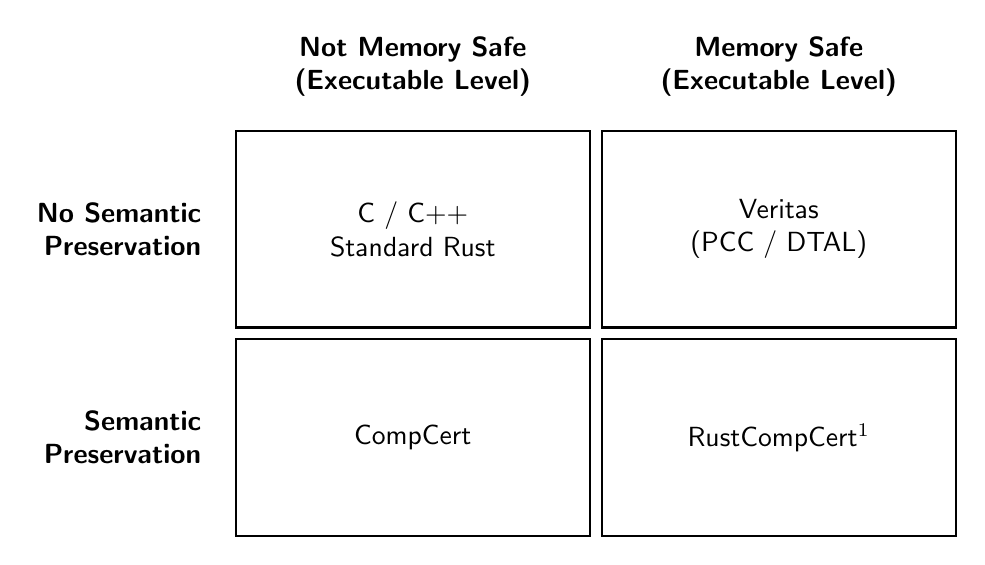
\begin{tikzpicture}[
        box/.style={draw, thick, minimum width=4.5cm, minimum height=2.5cm, align=center, font=\sffamily},
        header/.style={font=\sffamily\bfseries, align=center}
      ]

      \node[box] (c1r1) {C / C++ \\ Standard Rust};
      \node[box, right=0.12cm of c1r1] (c2r1) {Veritas \\ (PCC / DTAL)};
      \node[box, below=0.12cm of c1r1] (c1r2) {CompCert};
      \node[box, right=0.12cm of c1r2] (c2r2) {RustCompCert\footnotemark};

      \node[header, above=0.3cm of c1r1] {Not Memory Safe\\(Executable Level)};
      \node[header, above=0.3cm of c2r1] {Memory Safe\\(Executable Level)};

      \node[header, left=0.3cm of c1r1, align=right] {No Semantic\\Preservation};
      \node[header, left=0.3cm of c1r2, align=right] {Semantic\\Preservation};
    \end{tikzpicture}
  }
  \caption{A taxonomy of systems programming toolchains based on their executable-level guarantees.}
  \label{fig:safety-sem-taxonomy}
\end{figure}
\footnotetext{RustCompCert \cite{RustCompCert} is an ongoing project to verify an end-to-end compiler for the Rust programming language, but it currently only focuses on a small sequential subset of the language.}


Together, these components support the core question of the dissertation: whether a small systems-language toolchain can realise the trust model suggested by proof-carrying code, with an untrusted compiler whose low-level output is independently checked before execution. The dissertation evaluates this along two main axes:

\componentblock{Trust architecture}{Can the relevant low-level safety properties of compiled programs be checked independently at the DTAL level, and does the verifier remain small enough to audit without access to the source code or compiler state?}
\componentblock{Expressiveness and practicality}{Can the source language support realistic imperative, systems-oriented programs while retaining automatic verification?}


\chapter{Preparation}\label{ch:prep}

This chapter gives the background needed to understand the design of Veritas: the type-system machinery used to express safety properties, the related verification systems that informed the design, and the engineering decisions that fix the project's trust boundary. The aim is to establish only the theory and design context needed for the implementation that follows.

\section{Background}\label{sec:background}

\subsection{Type systems and safety}

The fundamental theorem that connects type systems to safety is \emph{type soundness}: a well-typed program cannot `go wrong' at runtime~\cite{Milner1978Theory}. Wright and Felleisen formalised this via the \emph{progress} and \emph{preservation} lemmas~\cite{Wright1994Syntactic}:

\begin{center}
\small
\begin{tabularx}{0.94\textwidth}{>{\raggedright\arraybackslash}p{0.22\textwidth} >{\raggedright\arraybackslash}X}
\toprule
\textbf{Progress} & If $\emptyset \vdash e : \tau$, then either $e$ is already a value, or there exists some expression $e'$ such that $e \to e'$. \\
\textbf{Preservation} & If $\emptyset \vdash e : \tau$ and $e \to e'$, then $\emptyset \vdash e' : \tau$. \\
\bottomrule
\end{tabularx}
\end{center}

\noindent Starting from a well-typed program, repeated evaluation can neither get stuck in an ill-defined intermediate state (progress) nor escape the guarantees expressed by its type (preservation). In practice, this is the formal basis for claims such as ``a well-typed array access cannot go out of bounds''.

The relevant distinction for Veritas is whether a type system can express facts about values, not only broad categories of values. Ordinary type systems classify values as integers, booleans, pointers, or polymorphic structures. Refinement and dependent type systems can also state that a particular integer is positive, that an index is in bounds, or that an array has a fixed length.

\subsection{Dependent types and refinement types}\label{sec:dependent-types}

\term{Dependent types} allow types to depend on terms. The canonical example is a vector type indexed by its length, $\mathrm{Vec}(A, n)$. A lookup function can require in its type that the index is valid:
\[
  \mathrm{lookup} :
  \mathrm{Vec}(A,n) \to
  \{i\!:\!\mathtt{int} \mid 0 \le i < n\} \to A
\]
Full dependent type systems, such as those in Coq and Agda~\cite{Bove2009Agda}, can express arbitrary propositions as types, but this generality comes at a cost: type checking is expensive and may require the programmer to construct explicit proof terms.

\term{Refinement types}~\cite{Rondon2008Liquid} are a practical restriction of full dependent types. A base type is decorated with a logical predicate drawn from a decidable logic, for example $\{v\!:\!\mathtt{int} \mid v > 0\}$. Subtyping between refinement types reduces to logical implication:
\[
  \{v\!:\!\mathtt{int} \mid P(v)\}
  <:
  \{v\!:\!\mathtt{int} \mid Q(v)\}
  \quad\text{when}\quad
  P(v) \Rightarrow Q(v)
\]
This turns refinement subtyping into an SMT obligation.

A particularly useful special case is the \term{singleton type}, written $\mathtt{int}(n)$, which is inhabited by exactly the integer $n$. Singleton types arise naturally from Xi and Pfenning's work on Dependent ML~\cite{Xi1999DML}, where integer index expressions are used to track array sizes and loop bounds. Singleton types can propagate exact values through arithmetic:
\[
  \begin{array}{rcl}
    x &:& \mathtt{int}(3) \\
    y &:& \mathtt{int}(5) \\
    x + y &:& \mathtt{int}(8)
  \end{array}
\]
This enables compile-time verification of array bounds when indices are statically known.

\subsection{Bidirectional type checking}

Bidirectional type checking~\cite{Pierce2000Local} structures type checking into two mutually recursive judgements:

\begin{center}
\small
\begin{tabularx}{0.94\textwidth}{>{\raggedright\arraybackslash}p{0.25\textwidth} >{\raggedright\arraybackslash}X}
\toprule
\textbf{Type checking} & Verifies that expression $e$ has expected type $\tau$: $\Gamma \vdash e \leftarrow \tau$. \\
\textbf{Type synthesis} & Infers a type $\tau$ for expression $e$: $\Gamma \vdash e \Rightarrow \tau$. \\
\bottomrule
\end{tabularx}
\end{center}
\noindent The two modes are connected by a subsumption rule:
$$
  \frac{\Gamma \vdash e \Rightarrow \sigma \quad \sigma <: \tau}{\Gamma \vdash e \leftarrow \tau}
$$
For refinement types, synthesis can produce precise local facts: integer literals synthesise singleton types, and arithmetic synthesises refinements relating the result to its operands. Checking then verifies subtyping against the expected type. In Veritas, programmers annotate function boundaries and mutable declarations; intermediate refinements are inferred.

The same structure also threads the typing context through the judgements, reflecting mutable assignments and newly learned refinement propositions.

\subsection{SMT-based verification}
\label{sec:smt-based-ver}

Satisfiability Modulo Theories (SMT) solvers check satisfiability of formulae over richer logics than propositional SAT. Veritas uses Z3~\cite{DeMoura2008Z3} for linear integer arithmetic, arrays, uninterpreted functions, and bounded quantifiers over array specifications.

The technique for using an SMT solver as a refinement type checker is \term{proof by refutation}~\cite{Rondon2008Liquid}. To check whether $\phi \vdash P$ holds, Veritas checks whether $\phi \wedge \lnot P$ is unsatisfiable:

\[
  \phi \vdash P
  \quad\text{iff}\quad
  \phi \wedge \lnot P \text{ is unsatisfiable}
\]

This approach means that proof obligations are discharged automatically: the programmer supplies type annotations, function contracts, and loop invariants, but never constructs proof terms. In Veritas, the SMT solver is invoked for refinement subtyping, array bounds verification, and function contract verification at call sites and return points.

\subsection{Type-preserving compilation and proof-carrying code}\label{sec:type-pres-background}

Conventional compilers erase types after type checking, discarding the safety guarantees established by the type system. The generated machine code is subsequently trusted on the basis that the compiler is correct, an assumption that is difficult to verify for large, complex compilers. Type-preserving compilation~\cite{Morrisett1999SystemF} retains type information through every intermediate representation in the pipeline. This enables the property that the compiled output can be independently verified without trusting the compiler. If a bug in the compiler produces type-incorrect code, the type annotations on the output will be inconsistent, and the verifier will reject it.

The idea of shipping machine code together with a checkable proof of its safety was formalised by Necula as proof-carrying code (PCC)~\cite{Necula1997PCC}. In PCC, the code producer generates executable code and a safety proof; the code consumer checks the proof against a safety policy before execution. Type-preserving compilation can be seen as a particular instance of PCC where the `proof' takes the form of type annotations.

\subsection{Dependently Typed Assembly}\label{sec:dtal-background}

Xi and Harper introduced DTAL as a target for type-preserving compilation from DML and Xanadu~\cite{Xi1999DML,Xi2000Xanadu}. DTAL augments assembly with two key forms of type annotation:
\begin{itemize}
  \item \textbf{Label signatures}: each basic block entry point is annotated with existentially quantified index variables and the types expected for each register on entry, enabling modular, block-by-block verification.
  \item \textbf{Register types}: types may depend on index variables, so that a register's type tracks its exact value (e.g., $\mathtt{int}(i)$) or the size of an array it points to (e.g., $\mathtt{int\;array}(n)$).
\end{itemize}

\noindent A DTAL loop header binds index variables and declares register types in terms of them:

\begin{verbatim}
  loop:  {m:nat, n:nat | m <= n, i:nat}
         [r1: int array(m), r2: int array(n), r3: int(m), r4: int(i)]
         sub   r5, r4, r3       // r5 <- i - m
         bgte  r5, finish       // if i >= m, exit
         load  r5, r1(r4)       // safe: i < m
         store r2(r4), r5       // safe: i < n (since m <= n)
         add   r4, r4, 1
         jmp   loop
\end{verbatim}

\noindent The branch \texttt{bgte r5, finish} refines the type state: on the fall-through path, the type system knows $i < m$, which makes the subsequent \texttt{load} and \texttt{store} provably safe without any runtime bounds check. Xi and Harper proved that well-typed DTAL programs cannot violate the constraints of the type system.

Veritas implements its own DTAL variant based on Xi and Harper's design, extended to support the Veritas refinement type system and x86-64. The compiler translates source through a typed intermediate representation (TIR) to DTAL, preserving refinement types at each stage, and finally emits x86-64 machine code as an ELF executable. Hereafter, `DTAL' refers to this Veritas-specific variant unless otherwise noted; the original is referred to as `Xi and Harper's DTAL'.

\section{Related work and design influences}
\label{sec:related-work}

Veritas combines automated refinement checking, systems-language design, and proof-carrying code. The systems below matter because each fixes a different point in the design space: automation, expressiveness, systems orientation, or low-level trust.

\subsection{Refinement types and automated verification}
Liquid Haskell~\cite{Vazou2014Refinement} and Liquid Types~\cite{Rondon2008Liquid} provide the main precedent for SMT-backed refinement checking. Dafny~\cite{Leino2010Dafny} similarly uses SMT solving for imperative contracts and loop invariants. Veritas borrows this style of automatic proof discharge, but preserves the resulting constraints down to assembly rather than erasing them after source-level verification.

\subsection{Foundational and dependent verification}
F*~\cite{Swamy2016Dependent} and RefinedC~\cite{Sammler2021RefinedC} offer stronger theoretical foundations through dependent types or separation logic. RefinedC, for example, produces machine-checked Coq proofs for existing C code. Veritas deliberately accepts a weaker foundation, SMT-backed checking rather than foundational proof, to keep proof obligations automatic once specifications are supplied.

\subsection{Verifiable systems languages}
ATS (Applied Type System)~\cite{Xi2003Applied} is the closest predecessor in spirit: it targets systems programming with dependent types and zero runtime overhead. The key difference is architectural. ATS proves properties at compile time and then emits C, leaving the ATS and C compilers in the TCB. Veritas instead preserves types into DTAL so that the low-level target can be checked independently.

The recurring difference is not whether verification is possible, but where the evidence is checked and what remains trusted after compilation. Figure~\ref{fig:verification-landscape} summarises the trade-off between expressiveness and automation across the systems discussed above.

\begin{figure}[H]
  \centering
  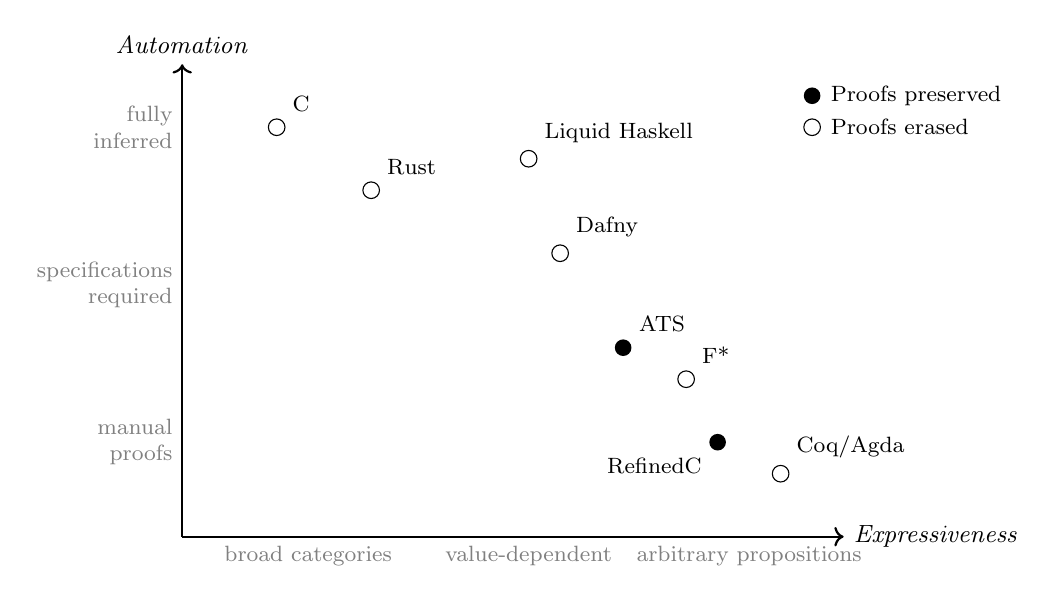
\begin{tikzpicture}[
      every node/.style={font=\small},
      filled/.style={circle, fill=black, inner sep=0pt, minimum size=6pt},
      hollow/.style={circle, draw=black, fill=white, inner sep=0pt, minimum size=6pt},scale=0.8
    ]
    \draw[->, thick] (0,0) -- (10.5,0) node[right] {\textit{Expressiveness}};
    \draw[->, thick] (0,0) -- (0,7.5) node[above] {\textit{Automation}};

    \node[below left, font=\footnotesize] at (0,0) {};
    \node[below, font=\footnotesize, text=gray] at (2,0) {broad categories};
    \node[below, font=\footnotesize, text=gray] at (5.5,0) {value-dependent};
    \node[below, font=\footnotesize, text=gray] at (9,0) {arbitrary propositions};
    \node[left, font=\footnotesize, text=gray, align=right] at (0,1.5) {manual\\proofs};
    \node[left, font=\footnotesize, text=gray, align=right] at (0,4) {specifications\\required};
    \node[left, font=\footnotesize, text=gray, align=right] at (0,6.5) {fully\\inferred};

    \node[hollow, label={[font=\footnotesize]above right:C}] at (1.5,6.5) {};

    \node[hollow, label={[font=\footnotesize]above right:Rust}] at (3,5.5) {};

    \node[hollow, label={[font=\footnotesize]above right:Liquid Haskell}] at (5.5,6) {};

    \node[hollow, label={[font=\footnotesize]above right:Dafny}] at (6,4.5) {};


    \node[filled, label={[font=\footnotesize]above right:ATS}] at (7,3) {};

    \node[hollow, label={[font=\footnotesize]above right:F*}] at (8,2.5) {};

    \node[filled, label={[font=\footnotesize]below left:RefinedC}] at (8.5,1.5) {};

    \node[hollow, label={[font=\footnotesize]above right:Coq/Agda}] at (9.5,1) {};

    \node[filled, label={[font=\footnotesize]right:Proofs preserved}] at (10,7) {};
    \node[hollow, label={[font=\footnotesize]right:Proofs erased}] at (10,6.5) {};

  \end{tikzpicture}
  \caption{Verification systems positioned by expressiveness of their type/specification language and degree of automation.}
  \label{fig:verification-landscape}
\end{figure}

\section{Requirements and success criteria}\label{sec:requirements-anal}

The requirements define what counts as success for Veritas: the language must express useful safety properties, the compiler must preserve evidence for those properties, and the generated low-level code must be checkable independently of the compiler. They were categorised using the MoSCoW method to keep the project focused on type-preserving compilation and independent low-level verification.

\begin{table}[H]
  \centering
  \small
  \begin{tabularx}{0.94\textwidth}{>{\raggedright\arraybackslash}p{0.16\textwidth} >{\raggedright\arraybackslash}X}
    \hline
    \textbf{Priority} & \textbf{Requirements} \\
    \hline
    Must-have & Variables, control flow, functions, arrays, refinement and singleton types; SMT-backed checking; type-preserving compilation to DTAL; a standalone verifier for generated assembly. \\
    Should-have & Native x86-64 ELF generation; function contracts with postconditions and quantified specifications; tests for accepted safe programs and rejected unsafe programs. \\
    Could-have & Backend optimisations; structs; generics; a full ownership model; a DTAL interpreter. \\
    Won't-have & A machine-checked compiler correctness proof; concurrency verification; information-flow or cryptographic verification. \\
    \hline
  \end{tabularx}
  \caption{MoSCoW requirements.}
  \label{tab:moscow-requirements}
\end{table}

\begin{center}
\small
\begin{tabularx}{0.94\textwidth}{>{\raggedright\arraybackslash}p{0.22\textwidth} >{\raggedright\arraybackslash}X}
\toprule
\textbf{Success criterion} & \textbf{Meaning} \\
\midrule
Expressiveness & Source-level safety properties can be expressed. \\
Preservation & Safety evidence is preserved through compilation to DTAL. \\
Independent rejection & Unsafe generated low-level code is rejected independently of the compiler. \\
Executable output & Accepted programs can be emitted and run as x86-64 ELF binaries. \\
\bottomrule
\end{tabularx}
\end{center}

\section{Design decisions}\label{sec:design-decisions}

The central design task was to realise this trust architecture without making the source language unusable or the trusted backend too large.

\subsection{Trust model and compiler architecture}

A central architectural decision is that the compiler is \textit{untrusted}. Rather than proving the compiler correct, Veritas relies on a standalone verifier that re-checks the compiler's low-level output. Compiler bugs should therefore cause rejection, not unsafely accepted code. Figure~\ref{fig:trust-pipeline} shows the resulting boundary: type information flows through the compiler, but trust begins only at the verifier and direct encoder.

The implementation moved the verification boundary progressively lower: first checking virtual DTAL, then physical DTAL after register allocation, and finally keeping the runtime small enough to audit by inspection, with a bare-metal target removing the OS from the TCB.

\begin{figure}[H]
  \centering
  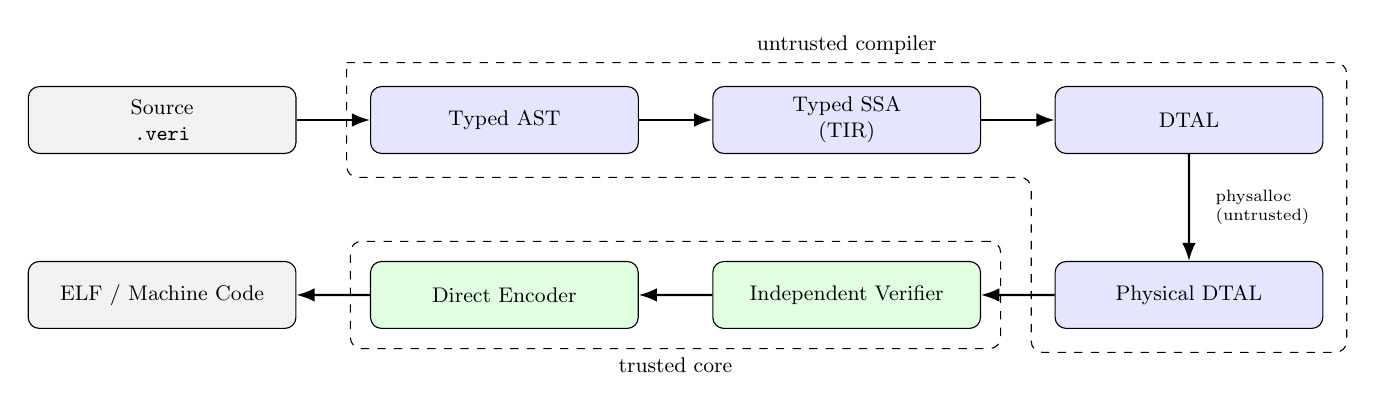
\begin{tikzpicture}[
      scale=0.85,
      transform shape,
      node distance=0.9cm and 1.1cm,
      box/.style={draw, rounded corners, minimum height=1.0cm, minimum width=4.0cm, align=center, font=\small},
      typed/.style={box, fill=blue!10},
      untyped/.style={box, fill=gray!10},
      trusted/.style={box, fill=green!12},
      arrow/.style={-Latex, thick}
    ]
    \node[untyped] (src) {Source\\\texttt{.veri}};
    \node[typed, right=of src] (tast) {Typed AST};
    \node[typed, right=of tast] (tir) {Typed SSA\\(TIR)};
    \node[typed, right=of tir] (dtal) {DTAL};

    \node[typed, below=1.6cm of dtal] (phys) {Physical DTAL};
    \node[trusted, left=of phys] (verifier) {Independent Verifier};
    \node[trusted, left=of verifier] (encoder) {Direct Encoder};
    \node[untyped, left=of encoder] (elf) {ELF / Machine Code};

    \draw[arrow] (src) -- (tast);
    \draw[arrow] (tast) -- (tir);
    \draw[arrow] (tir) -- (dtal);
    \draw[arrow] (dtal) -- node[right=0.35cm, font=\scriptsize, align=left, fill=white, inner sep=1pt] {physalloc\\(untrusted)} (phys);
    \draw[arrow] (phys) -- (verifier);
    \draw[arrow] (verifier) -- (encoder);
    \draw[arrow] (encoder) -- (elf);

    \draw[dashed, rounded corners]
    ([xshift=-0.35cm,yshift=0.35cm]tast.north west) --
    ([xshift=0.35cm,yshift=0.35cm]dtal.north east) --
    ([xshift=0.35cm,yshift=-0.35cm]dtal.south east) --
    ([xshift=0.35cm,yshift=-0.35cm]phys.south east) --
    ([xshift=-0.35cm,yshift=-0.35cm]phys.south west) --
    ([xshift=-0.35cm,yshift=-0.35cm]dtal.south west) --
    ([xshift=-0.35cm,yshift=-0.35cm]tast.south west) --
    ([xshift=-0.35cm,yshift=0.35cm]tast.north west);
    \node[font=\small, above] at ([yshift=0.35cm]tir.north) {untrusted compiler};
    \node[draw, dashed, rounded corners, fit=(verifier)(encoder), inner sep=0.25cm,
      label={[font=\small]below:trusted core}] {};
  \end{tikzpicture}
  \caption{Veritas compilation pipeline and trust boundary. The final design verifies physical DTAL, so register allocation and instruction selection remain outside the trusted core.}
  \label{fig:trust-pipeline}
\end{figure}

\subsection{Language and target choices}\label{sec:prep-language-target}

\prepblock{Source language}{Veritas is a small imperative language with C-like syntax, inspired by Xi and Harper's Xanadu. It supports integers, booleans, fixed-size arrays, mutable and immutable variables, loops, and functions. The type system adds singleton types, refinement types, contracts, bounded quantifiers, and loop invariants.}

\prepblock{Bounded quantification}{Scalar refinements can prove facts about individual values, but algorithms such as binary search need array-wide properties such as sortedness. A precondition such as $\mathbf{forall}\ i\ \mathbf{in}\ 0..n\ \{\ \mathit{arr}[i] \le \mathit{arr}[i + 1]\ \}$ expresses such properties while keeping verification close to SMT-friendly fragments.}

\prepblock{DTAL target}{The target language is a variant of Xi and Harper's DTAL~\cite{Xi2001DTAL}, extended for Veritas refinements and x86-64. The core instruction set is deliberately RISC-like: simple instructions are easier to type, verify, and map from the SSA-style intermediate representation. DTAL then adds register type annotations, embedded constraint assertions, and declared type states at basic block entries.}

\prepblock{Physical register model}{I also defined DTAL with its own \term{physical register model} (registers \texttt{r0}--\texttt{r12}, \texttt{sp}, \texttt{fp}, \texttt{lr}) that maps directly to x86-64 registers. This allows verification to occur \term{after} register allocation: the register allocator is untrusted, and its output is verified before the final encoding to x86-64.}

\prepblock{Direct encoding}{Rather than emitting assembly text and invoking NASM or GAS, Veritas encodes x86-64 instructions directly as bytes. This keeps an external assembler out of the TCB and enables direct execution on the development machine. The trusted path below physical DTAL is intentionally small: a one-to-one instruction mapping, a byte encoder, and an ELF generator.}

\subsection{Design challenges}\label{sec:design-challenges}

Four design challenges shaped the implementation:

\challengeblock{Mutable variables and refinement types}{Refinement type systems such as Liquid Haskell operate over immutable bindings, where a variable's type is fixed at its definition. Supporting mutation introduces a soundness hazard: after \texttt{x = e}, any refinement mentioning \texttt{x} may be invalidated.}{The solution adopted, \term{master types}, required designing the mutable context $\Delta$ to track both a current type and a fixed master type, with a subtyping check on every assignment.}{This keeps refinements sound in the presence of assignment.}

\challengeblock{Verification after register allocation}{The initial system verified DTAL with virtual registers and then trusted the x86-64 lowering ($\sim$1,100 lines of register allocation, instruction selection, and encoding).}{Redesigning the pipeline to verify \term{after} register allocation required a physical DTAL register model, an untrusted allocation pass, a direct encoder, and verifier support for physical instructions.}{This reduced the trusted backend code to $\sim$300 lines.}

\challengeblock{Type preservation across SSA join points}{At phi nodes in the SSA intermediate representation, two singleton types from different branches (e.g., $\mathtt{int}(3)$ and $\mathtt{int}(7)$) must be joined. Widening to the base type $\mathtt{int}$ loses refinement information, making downstream bounds proofs impossible.}{The solution was to attach \term{existential constraints} to phi nodes, encoding that the value satisfies a constraint without fixing it to a concrete value.}{This mechanism was not part of Xi and Harper's original DTAL design and required extending both the TIR and the verifier.}

\challengeblock{SMT encoding of array properties}{Verifying array-manipulating programs requires reasoning about array contents, which involves quantified formulae. These fall outside the decidable quantifier-free fragment of linear integer arithmetic.}{The design restricted quantifiers to \term{bounded} forms ($\mathbf{forall}\ x\ \mathbf{in}\ a..b$), which Z3's E-matching heuristics handle reliably in practice.}{This excludes unbounded quantification, but maintains the automatability of verification.}

\section{Project management and starting point}
\label{sec:software-eng-methodology}

\prepblock{Development process}{The implementation followed an incremental pipeline-first strategy. I first built an end-to-end compiler for integer arithmetic, then extended the same path with arrays, mutation, refinements, contracts, and quantifiers. Each feature was accompanied by positive tests that should compile and negative tests that should be rejected with a specific error.}

\prepblock{Engineering process and tools}{Version control was managed using Git, with short-lived feature branches merged into the main branch. A GitHub Actions CI pipeline ran on each push, enforcing \texttt{cargo fmt}, \texttt{cargo clippy}, example validation, and the test suite on Ubuntu Linux and macOS. The project was implemented in Rust; the frontend type checker and DTAL verifier use Z3 via the \texttt{z3} Rust crate, and \texttt{im} provides persistent data structures for typing contexts.}

\prepblock{Professional practice}{The project used open-source dependencies whose licences were checked before inclusion and are listed where they affect the implementation boundary. The evaluation uses generated programs, authored examples, and public benchmark kernels rather than personal data or human-subject data, so data-protection and human-subject concerns are minimal. The main consequence of the work is research-facing: it explores how safety evidence can be preserved into low-level code, which could reduce trust in compiler infrastructure if developed further.}

\prepblock{Starting point}{I began with introductory knowledge of dependent type theory and verification languages, and was introduced to refinement types through Xi and Harper's DTAL. No external compiler or verifier code was used. The main new areas were Rust, SMT-backed type checking, Z3 theories, x86-64 encoding, bidirectional type checking, and the Xi et al. papers on DML, Xanadu, and DTAL.}


\chapter{Implementation}\label{ch:impl}
This chapter describes the implementation of the Veritas toolchain as a journey from source-level specifications to independently checked machine code. The implementation consists of a refinement-typed source language, a bidirectional frontend checker, a typed SSA intermediate representation, a DTAL backend, an independent verifier, a compact runtime, and a bare-metal unikernel target. The chapter first gives the repository and pipeline structure, then follows the path taken by safety evidence through the compiler and verifier. Finally, Section~\ref{sec:worked-example} traces a binary search program through the full pipeline.

\section{Repository overview}\label{sec:repo-overview}

The implementation is deliberately broad: it includes the source language, compiler pipeline, verifier, executable generator, runtime, and bare-metal target. The source code is organised as a single Rust crate. Table~\ref{tab:repo} gives the main implementation areas rather than every internal module.
\begin{table}[h]
  \centering
  \small
  \begin{tabularx}{0.96\textwidth}{>{\raggedright\arraybackslash}p{0.28\textwidth} r >{\raggedright\arraybackslash}X}
    \hline
    \textbf{Area}                         & \textbf{Lines}  & \textbf{Responsibility}                     \\
    \hline
    \texttt{src/common/}                       & 687             & Shared AST, typed AST, and type definitions \\
    \texttt{src/frontend/}                     & 7,856           & Lexer, parser, and bidirectional type checker \\
    \texttt{src/backend/}                      & 17,391          & TIR, DTAL, optimisation, allocation, encoding, ELF, runtime \\
    \texttt{src/verifier/}                     & 7,372           & Independent DTAL verifier                   \\
    \texttt{src/main.rs}, \texttt{src/pipeline.rs} & 1,013       & CLI and pipeline orchestration              \\
    Other crate and binary files               & 262             & Module glue and helper binary               \\
    \hline
    \textbf{Total (excl.\ tests)}              & \textbf{34,581} &                                          \\
    \hline
  \end{tabularx}
  \caption{Repository structure and measured non-test Rust line counts.}
  \label{tab:repo}
\end{table}

\noindent The compiler, verifier, runtime, direct encoder, and test suite were written from scratch for this project. Outside \texttt{src/}, the repository contains 85 positive example programs, 35 negative examples, 424 Rust unit tests, integration tests for example verification and DTAL tampering, and an evaluation harness. The main third-party crates are \texttt{z3}, \texttt{chumsky}, \texttt{im}, and \texttt{ariadne}; these support infrastructure rather than implementing the Veritas language, compiler, verifier, runtime, or encoder.

Veritas is exposed as a command-line compiler over \texttt{.veri} source files. The normal path type-checks the source program, lowers it through TIR and DTAL, optionally verifies the resulting DTAL, and emits a freestanding ELF executable. The most important user-facing modes are \texttt{--verify}, which performs independent DTAL verification before native output is accepted, \texttt{--verify-dtal}, which checks a standalone \texttt{.dtal} file without using the source compiler, and \texttt{--target-bare-metal}, which emits a Multiboot-compatible binary for QEMU. This interface matters for the trust story: the verifier is not just an internal pass hidden inside the compiler, but can be run directly on the low-level artefact that the compiler produced.

\subsection{Pipeline overview}
Figure~\ref{fig:pipeline} summarises the compilation pipeline. Each named representation is shown in sequence, and arrows indicate the transformations between them. Type annotations are preserved through TAST, TIR, and DTAL, and are no longer needed after DTAL verification and final encoding to x86-64.
\begin{figure}[h]
  \centering
  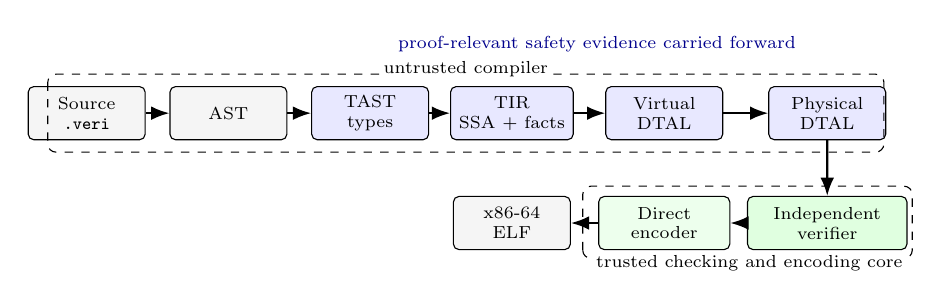
\begin{tikzpicture}[
      scale=0.9,
      transform shape,
      stage/.style={draw, rounded corners=2pt, minimum width=1.65cm, minimum height=0.75cm, align=center, font=\scriptsize},
      evidence/.style={stage, fill=blue!9},
      plain/.style={stage, fill=gray!8},
      verifier/.style={stage, fill=green!12, minimum width=2.25cm},
      trusted/.style={stage, fill=green!7, minimum width=1.85cm},
      pass/.style={font=\scriptsize, text=black!70, align=center},
      arrow/.style={-Latex, thick}
    ]
    \node[plain] (src) at (0,0) {Source\\\texttt{.veri}};
    \node[plain] (ast) at (2.0,0) {AST};
    \node[evidence] (tast) at (4.0,0) {TAST\\types};
    \node[evidence] (tir) at (6.0,0) {TIR\\SSA + facts};
    \node[evidence] (vdtal) at (8.15,0) {Virtual\\DTAL};
    \node[evidence] (pdtal) at (10.45,0) {Physical\\DTAL};
    \node[verifier] (verify) at (10.45,-1.55) {Independent\\verifier};
    \node[trusted] (enc) at (8.15,-1.55) {Direct\\encoder};
    \node[plain] (elf) at (6.0,-1.55) {x86-64\\ELF};

    \draw[arrow] (src) -- (ast);
    \draw[arrow] (ast) -- (tast);
    \draw[arrow] (tast) -- (tir);
    \draw[arrow] (tir) -- (vdtal);
    \draw[arrow] (vdtal) -- (pdtal);
    \draw[arrow] (pdtal) -- (verify);
    \draw[arrow] (verify) -- (enc);
    \draw[arrow] (enc) -- (elf);

    \draw[dashed, rounded corners=3pt]
      (-0.55,0.55) rectangle (11.25,-0.55);
    \node[font=\scriptsize, fill=white, inner sep=1pt] at (5.35,0.62) {untrusted compiler};

    \draw[dashed, rounded corners=3pt]
      (7.0,-2.05) rectangle (11.65,-1.03);
    \node[font=\scriptsize, fill=white, inner sep=1pt] at (9.35,-2.12) {trusted checking and encoding core};

    \node[font=\scriptsize, align=center, text=blue!55!black] at (7.2,0.98)
      {proof-relevant safety evidence carried forward};
  \end{tikzpicture}
  \caption{The Veritas compilation pipeline. Blue stages carry type and constraint evidence; verification occurs after register allocation.}
  \label{fig:pipeline}
\end{figure}

\section{Source language and frontend checker}\label{sec:source-language}

This section presents the syntax, typing rules, and frontend implementation of the Veritas source language. These define the first contract in the pipeline: any program accepted by the type checker satisfies the properties encoded in its types.

\subsection{Syntax}

Veritas is a first-order imperative language with refinement-carrying types, fixed-size arrays, references, contracts, loop invariants, and bounded quantified specifications. The main syntactic categories are:
{\small
\[
\renewcommand{\arraystretch}{1.09}
\begin{array}{@{}r@{\ }c@{\ }l@{\hspace{0.8em}}p{0.22\textwidth}@{}}
  T, \tau & ::= &
  \parbox[t]{0.63\textwidth}{
    $\textsf{unit} \,|\, \textsf{int} \,|\, \textsf{bool} \,|\, [T; N] \,|\, \textsf{\&}T \,|\, \textsf{\&mut } T \,|\, \textsf{int}(N) \,|\, \{ x:\textsf{int} \mid P \}$
  }
  & \textbf{(Types)} \\[2pt]
  c & ::= &
  \underline{n} \,|\, \textsf{true} \,|\, \textsf{false}
  & \textbf{(Base values)} \\[2pt]
  \textsf{aop} & ::= &
  \texttt{+} \,|\, \texttt{-} \,|\, \texttt{*} \,|\, \texttt{/} \,|\, \texttt{\%}
  \qquad \textsf{uaop} ::= \texttt{-}
  & \textbf{(Arith. ops)} \\[2pt]
  \textsf{cop} & ::= &
  \texttt{==} \,|\, \texttt{!=} \,|\, \texttt{<} \,|\, \texttt{<=} \,|\, \texttt{>} \,|\, \texttt{>=}
  & \textbf{(Comparison ops)} \\[2pt]
  \textsf{lop} & ::= &
  \texttt{\&\&} \,|\, \texttt{||} \,|\, \texttt{==>}
  \qquad \textsf{ulop} ::= \texttt{!}
  & \textbf{(Logical ops)} \\[2pt]
  e & ::= &
  \parbox[t]{0.63\textwidth}{
    $c \,|\, x \,|\, e \textsf{ aop } e \,|\, e \textsf{ cop } e \,|\, e \textsf{ lop } e \,|\, \textsf{ulop}\; e \,|\, \textsf{uaop}\; e \,|\, f(\overrightarrow{e}) \,|\, {}$\\
    $x[e_i] \,|\, \kw{if } e_\textsf{cond}\; \{B\}\; \kw{else } \{B'\} \,|\, [e_\textsf{val}; e_\textsf{size}]$
  }
  & \textbf{(Expressions)} \\[4pt]
  P & ::= &
  \parbox[t]{0.63\textwidth}{
    $e \textsf{ cop } e \,|\, P \textsf{ lop } P \,|\, \textsf{ulop}\; P \,|\, {}$\\
    $\kw{forall } x \kw{in } e_\textsf{start}..e_\textsf{end}\;\{P\} \,|\, \kw{exists } x \kw{in } e_\textsf{start}..e_\textsf{end}\;\{P\}$
  }
  & \textbf{(Propositions)} \\[4pt]
  S & ::= &
  \parbox[t]{0.63\textwidth}{
    $\kw{let } x:T = e; \,|\, \kw{let mut } x:T = e; \,|\, x = e; \,|\, x[e_i] = e; \,|\, \kw{return } e; \,|\, e; \,|\, {}$\\
    $\kw{if } e_\textsf{cond}\; \{B\}\; \kw{else } \{B'\} \,|\, \kw{if } e_\textsf{cond}\; \{B\} \,|\, {}$\\ 
    $\kw{for } x \kw{in } e_\textsf{start}..e_\textsf{end}\; \optclause{\textsf{invariant } P}\; \{B\} \,|\, \kw{while } e_\textsf{cond}\; \optclause{\textsf{invariant } P}\; \{B\}$
  }
  & \textbf{(Statements)} \\[4pt]
  D & ::= &
  \parbox[t]{0.63\textwidth}{
    $\kw{fn } f(x_1:T_1, \ldots)\; \rightarrow T_\textsf{ret}\; \optclause{\textsf{requires } P}\;\optclause{\textsf{ensures } P}\; \{B\}$
  }
  & \textbf{(Function defs)} \\[2pt]
  \textsf{Prog} & ::= &
  D^*
  & \textbf{(Program)} \\[2pt]
  B & ::= &
  S^*\; \optclause{e}
  & \textbf{(Blocks)}
\end{array}
\]
}

Here $n$ ranges over integer literals, $x$ and $f$ over identifiers, and $N$ over statically known integer expressions used for array sizes and singleton types. $P$ is the shared specification language for refinements, contracts, loop invariants, and bounded quantifiers.

\subsection{Typing contexts}\label{sec:typing-contexts}

The typing context is a tuple $(\phi, \Gamma, \Delta, \Sigma_F)$:

\begin{center}
\small
\begin{tabularx}{0.95\textwidth}{>{\raggedright\arraybackslash}p{0.12\textwidth} >{\raggedright\arraybackslash}X}
\toprule
\textbf{Part} & \textbf{Meaning} \\
\midrule
$\phi$ & A set of refinement propositions known to be true: assumptions from branch conditions, preconditions, and refinement types. \\
$\Gamma$ & An immutable variable environment mapping names to types ($x : \tau$). \\
$\Delta$ & A mutable variable environment mapping names to a \textit{current type} and a \textit{master type} ($x : (\tau_c, \tau_m)$). We write $(x: \tau_c) \in \Delta$ to extract the current type and $(x: \tau_m) \in \Delta$ for the master type. \\
$\Sigma_F$ & A global function signature environment, read-only after an initial pass. \\
\bottomrule
\end{tabularx}
\end{center}

\subsubsection{Master types}

The master type $\tau_m$ is set at declaration and never changes; the current type $\tau_c$ may be refined through assignments and control flow but must remain a subtype of $\tau_m$. Thus a mutable \texttt{let mut x: T = e} records $T$ as the master type, allows the current type to narrow, and checks every assignment against the master type. At control-flow joins, current types from each branch are merged, but the result must still remain below the master type. This prevents reassignment from invalidating refinements.

The interaction between master types and mutable variables is described in Section~\ref{sec:typechecker}.

\subsection{Context joining}\label{sec:context-joining}

At control-flow merge points (i.e., after \textbf{if-else} and loops), the typing contexts from each branch must be joined. The $\textsf{join}$ operation computes a least upper bound for each mutable variable's type and intersects the proposition sets:

\begin{center}
\small
\begin{tabularx}{0.96\textwidth}{>{\raggedright\arraybackslash}p{0.24\textwidth} >{\raggedright\arraybackslash}X}
\toprule
\textbf{Case} & \textbf{Join rule} \\
\midrule
Same singletons & $\textsf{int}(N) \sqcup \textsf{int}(N) = \textsf{int}(N)$. \\
Different singletons & $\textsf{int}(N_1) \sqcup \textsf{int}(N_2) = \textsf{int}$ where $N_1 \ne N_2$. \\
Refined types & $\{v \mid P\} \sqcup \{v \mid Q\} = \{v \mid P \vee Q\}$. \\
Singleton and refined & Promote the singleton to $\{v \mid v = N\}$, then disjoin with the refined type's predicate. \\
Refined and unrefined & $\{v \mid P\} \sqcup \textsf{int} = \textsf{int}$. \\
Arrays & $[\tau_1; N] \sqcup [\tau_2; N] = [\tau_1 \sqcup \tau_2; N]$. \\
Propositions ($\phi$) & Intersect, keeping only propositions provable in both branches. \\
\bottomrule
\end{tabularx}
\end{center}

\noindent When $\textsf{join}$ is used in expression rules (e.g., \textsc{T-If-Expr}), the same type-joining rules apply to the result types of both branches.

\subsection{Judgement forms}\label{sec:judgement-forms}

Throughout the typing rules, $\tau$ is used as the metavariable for types.

The type system uses the following bidirectional typing judgements:

\begin{center}
\small
\begin{tabularx}{0.96\textwidth}{>{\raggedright\arraybackslash}p{0.17\textwidth} >{\raggedright\arraybackslash}X}
\toprule
\textbf{Judgement} & \textbf{Meaning} \\
\midrule
Synthesis & $\phi; \Delta; \Gamma \vdash e \Rightarrow (\phi'; \Delta'; \tau)$ synthesises type $\tau$ for expression $e$, potentially updating the context. \\
Checking & $\phi; \Delta; \Gamma \vdash e \Leftarrow \tau : (\phi'; \Delta')$ checks that $e$ has type $\tau$. \\
Subtyping & $\phi \vdash \tau_1 <: \tau_2$ states that $\tau_1$ is a subtype of $\tau_2$ under assumptions $\phi$. \\
Provability & $\phi \vdash P$ states that proposition $P$ is valid under assumptions $\phi$, decided by SMT. \\
\bottomrule
\end{tabularx}
\end{center}

The checking and synthesis judgements are connected by subsumption: if an expression synthesises type $\tau_1$ and the expected type is $\tau_2$, checking succeeds when $\tau_1 <: \tau_2$.

\subsection{Subtyping rules}

The subtyping relation $\phi \vdash \tau_1 <: \tau_2$ is defined by structural rules (reflexivity, singleton-to-int widening, refined-to-int widening, array covariance, master type transparency; listed in full in Appendix~\ref{app:source-rules}) and SMT-backed refinement implication. In each SMT-backed case, the propositions in $\phi$ are asserted as assumptions, the goal is negated, and the solver is checked for unsatisfiability:

$$\frac{\phi \vdash P[N/x]}{\phi \vdash \textsf{int}(N) <: \{x: \textsf{int} \mid P\}} \quad (\textsc{Sub-Singleton-Refine})$$

\subsection{Expression typing rules}\label{sec:expr-typing-rules}

The expression rules are standard bidirectional rules with three Veritas-specific behaviours:

\begin{center}
\small
\begin{tabularx}{0.96\textwidth}{>{\raggedright\arraybackslash}p{0.25\textwidth} >{\raggedright\arraybackslash}X}
\toprule
\textbf{Construct} & \textbf{Typing behaviour} \\
\midrule
Arithmetic & Constant-folds singleton operands and otherwise synthesises a refinement relating the result to the operands. \\
Array indexing & Synthesises the index type, extracts its logical proposition, and sends the bounds obligation $0 \le i < N$ to SMT. \\
Conditionals & Checks each branch under the condition and its negation, then joins the resulting contexts and result types. \\
Function calls & Checks argument subtyping and discharges the callee precondition after substituting actual arguments for formals. \\
\bottomrule
\end{tabularx}
\end{center}

The full expression rules, including the auxiliary $\textsf{val}$ and $\textsf{prop}$ functions used to extract index values and carried propositions, are given in Appendix~\ref{app:source-rules}.

\subsection{Statement typing rules}\label{sec:stmt-typing-rules}

Statement checking updates the typing context according to the statement's effect. Assignments synthesise the new value's type, check it against the variable's master type, and update the current type in $\Delta$. Loops add range facts for the induction variable and check any invariant twice: once on entry, and once after the body with the next iteration's value substituted. The full statement rules are given in Appendix~\ref{app:source-rules}.

\subsection{Function contracts}

Programmers may declare preconditions ($\mathbf{requires}\ P$) and postconditions ($\mathbf{ensures}\ P$) on functions. At each call site, the type checker verifies the precondition with actual arguments substituted for formals; at each return, it checks the return type and verifies the postcondition with the returned expression substituted for $\mathtt{result}$.

\subsection{Quantified specifications}

The constraint language supports bounded universal and existential quantifiers, plus implication, in specification positions only. This is enough to express array-wide properties such as sortedness and elementwise non-negativity without making quantifiers part of runtime computation. A useful implementation feature is \textit{refinement lifting}: an array typed as $[\{v\!:\!\textsf{int} \mid v \ge 0\}; N]$ automatically contributes the quantified fact $\forall i \in [0, N).\; \mathit{arr}[i] \ge 0$ when the array is in scope.

\subsection{Frontend implementation}\label{sec:frontend}

\subsubsection{Lexing and parsing}

The lexer and parser are built using \texttt{chumsky}. The frontend uses two expression parsers: a full parser for runtime expressions, and a restricted parser for refinement type annotations. This keeps type-position syntax unambiguous while reusing the same arithmetic and comparison language for specifications.

\subsubsection{Type checker}\label{sec:typechecker}

The type checker is the most substantial frontend component. It implements the bidirectional typing rules described in Section~\ref{sec:source-language}, using Z3 as an SMT oracle.

\detailhead{Architecture}The type checker is structured around the \texttt{TypingContext} $(\phi, \Gamma, \Delta, \Sigma_F)$ defined in Section~\ref{sec:typing-contexts}. Contexts are immutable values: each judgement takes a context as input and returns an updated context as output. The \texttt{im} crate makes branch cloning cheap through persistent data structures.

The type checker operates in two passes. The first collects all function signatures into $\Sigma_F$, enabling mutual recursion and allowing functions to be defined in any order. The second type-checks each function body against its signature.

\pagebreak[3]
\detailhead{Bidirectional checking}The implementation provides an explicit synthesis combinator, \texttt{synth\_expr}. Integer literals produce singleton types ($\mathtt{int}(n)$), variable lookups return the type from $\Gamma$ or $\Delta$, and arithmetic operations use \texttt{join\_op}. Checking first synthesises a type, then verifies by SMT-backed subtyping that it conforms to the expected type.

Statement checking (\texttt{check\_stmts}) updates the typing context according to each statement's effect: \texttt{let} bindings extend $\Gamma$ or $\Delta$, assignments update the current type in $\Delta$, and loops are checked by proving that their invariants hold on entry and are preserved by the body, as described in the statement typing rules for loops in Section~\ref{sec:stmt-typing-rules}.

\begin{verbatim}
synth_expr(ctx, expr) -> Result<(typed_expr, ty), TypeError>
check_stmt(ctx, stmt) -> Result<(typed_stmt, ctx'), TypeError>
check_stmts(ctx, stmts) -> Result<(typed_stmts, ctx'), TypeError>
check_program(program) -> Result<typed_program, TypeError>
\end{verbatim}

\detailhead{Singleton propagation and refinement synthesis}When both operands of an arithmetic operation are singletons, the checker folds at the type level: $\mathtt{int}(a) \oplus \mathtt{int}(b) = \mathtt{int}(a \oplus b)$. Otherwise it constructs a fresh refinement $\{v\!:\!\mathtt{int} \mid v = e_L \oplus e_R\}$, giving downstream stages enough information to verify computed indices such as \texttt{lo + (hi - lo) / 2}.

\detailhead{SMT oracle}\label{sec:smt-oracle}The SMT oracle wraps Z3 and provides a single entry point: $\texttt{is\_provable}(\phi, P)$. It asserts the assumptions, asserts $\lnot P$, and checks for unsatisfiability. Integer and boolean expressions map to the corresponding Z3 sorts; arrays use Z3 arrays; bounded quantifiers are translated to implications over native Z3 quantifiers.

The oracle also performs the refinement lifting described above, so element-level array refinements remain available to quantified proof obligations.

\detailhead{Error reporting}Type errors are structured \texttt{TypeError} values carrying source spans, expected and actual types, and contextual information. A reporting module formats these with \texttt{ariadne}, including the assumptions and failed proof goal where relevant.

\section{Typed intermediate representation and preservation}\label{sec:middle-end}

\subsection{Typed Intermediate Representation (TIR)}

The TIR is a typed SSA (Static Single Assignment) intermediate representation. Each function is a control-flow graph of basic blocks; each block contains a sequence of three-address instructions followed by a terminator (jump, conditional branch, or return). Every instruction carries type annotations from the source-level type checker, and every virtual register is defined exactly once.

\begin{center}
\small
\begin{tabularx}{0.96\linewidth}{@{}p{0.24\linewidth}X@{}}
\toprule
\textbf{Design choice} & \textbf{Implementation role} \\
\midrule
SSA form & Liveness analysis for register allocation is straightforward, and each virtual register has a single definition, so its type annotation has an unambiguous meaning. \\
Phi nodes & Control-flow joins become explicit program points where refinements from different predecessors can be joined rather than discarded silently. \\
Existential phi constraints & Loop counters and refined mutable variables can retain symbolic facts such as $\exists v.\; \mathtt{int}(v) \;\mathbf{where}\; (v \ge \mathit{start} \wedge v < \mathit{end})$, without fixing a concrete value. \\
\bottomrule
\end{tabularx}
\end{center}

The existential constraint is the key extension beyond ordinary SSA. It avoids the information loss that would occur if loop-carried values were simply widened to their base type.

\subsubsection{Representative instruction forms}

TIR is designed to sit close to both the typed source language and the DTAL backend. The implementation's instruction set includes ownership and region operations, but the core forms relevant to the compilation pipeline are summarised in Figure~\ref{fig:tir-syntax}.

In concrete terms, a TIR function stores its parameters, pre/postconditions, and a map of basic blocks; each block contains entry phi nodes, ordinary instructions, a terminator, and an entry register state. This makes the representation explicit enough for code generation to be largely structural, while still retaining the source-level type information needed for later verification.

\subsection{Lowering from TAST to TIR}

The lowering pass translates the typed AST to TIR. A \texttt{LoweringContext} maps source variables to virtual registers, tracks the current basic block, lowers statements in order, lowers any trailing expression to a result register, and packages the resulting blocks, phi nodes, entry states, and translated contracts into a \texttt{TirFunction}.

\subsubsection{Syntax-directed translation}

Lowering is syntax-directed: each typed source construct becomes a small SSA fragment while threading the variable-to-register map. Variable uses read the current register; \texttt{let} creates a fresh register; assignment updates the map so later uses see the new SSA value. Integer literals become \texttt{LoadImm}; arithmetic and comparisons become \texttt{BinOp} or \texttt{UnaryOp}; array operations become \texttt{ArrayLoad} and \texttt{ArrayStore} with explicit bounds constraints; calls carry argument registers, passing modes, ownership transfer, and result types. Conditionals introduce branch and merge blocks; loops introduce entry, header, body, and exit blocks with header phi nodes.

\begin{figure}[H]
\centering
\begin{verbatim}
block       ::= phi_node* instruction* terminator

phi_node    ::= PhiNode { dst, ty, incoming, existential_constraint? }

instruction ::= LoadImm { dst, value, ty }
              | Copy { dst, src, ty }
              | BinOp { dst, op, lhs, rhs, ty }
              | UnaryOp { dst, op, operand, ty }
              | ArrayLoad { dst, base, index, element_ty, 
                            bounds_constraint }
              | ArrayStore { base, index, value,
                             bounds_constraint }
              | Call { dst?, func, args, arg_types, arg_kinds, 
                       ownership, result_ty }
              | AssumeConstraint { constraint }
              | AssertConstraint { constraint }

terminator  ::= Jump { target }
              | Branch { cond, true_target, false_target,
                         true_constraint, false_constraint }
              | Return { value?, ownership }
\end{verbatim}
\caption{Representative TIR forms as defined in the implementation. The full implementation also includes ownership-transfer, borrowing, region, and allocation instructions.}
\label{fig:tir-syntax}
\end{figure}

\subsubsection{Ownership and borrowing through the pipeline}

Ownership is not treated as only a frontend check. The frontend tracks moved bindings, active borrows for each owner, reverse links from borrow variables back to their owners, and lexical borrow scopes. Creating \texttt{\&x} records a shared borrow; creating \texttt{\&mut x} requires no live borrow of the owner; moving or dropping an owner is rejected while conflicting borrows are still live.

\begin{center}
\small
\begin{tabularx}{\linewidth}{@{}p{0.19\linewidth}X@{}}
\toprule
\textbf{Stage} & \textbf{Ownership evidence kept explicit} \\
\midrule
Source checker & Binding state records owners, moved values, active shared borrows, active mutable borrows, and borrow scopes. \\
TIR & \texttt{MoveOwned}, \texttt{DropOwned}, \texttt{BorrowShared}, \texttt{BorrowMut}, and \texttt{BorrowEnd} make ownership changes visible before register allocation. \\
DTAL & \texttt{move\_owned}, \texttt{alias\_borrow}, \texttt{borrow\_mut}, \texttt{borrow\_end}, and \texttt{drop\_owned} expose the same events at the typed assembly level. \\
Verifier & Object identities, owned registers, and live borrows are checked after register allocation, so an incorrect backend cannot silently duplicate or alias ownership. \\
\bottomrule
\end{tabularx}
\end{center}

This gives ownership a low-level trust boundary. The verifier rejects duplicated owners, mutable borrows while aliases are live, and moves or drops while an active borrow remains. These checks run over allocated DTAL, at the same point as array-bounds and contract checks.

\subsubsection{Control flow}

\textbf{Conditionals} lower in the standard SSA style, except that each branch edge carries the logical fact derived from the condition. Thus \texttt{if x > 0} gives $x > 0$ on the taken edge and $\neg(x > 0)$ on the other. Phi nodes are inserted only where the assigned register differs.

\textbf{For-loops} use entry, header, body, and exit blocks. The induction variable is a header phi node with an existential range constraint $[\mathit{start}, \mathit{end})$, and mutable variables in scope receive loop-carried phi nodes. \textbf{While-loops} use the same shape, but rely on the translated branch condition and any programmer-supplied invariant rather than an explicit interval constraint.

\subsubsection{Constraint propagation}

Branch conditions are translated into the TIR constraint language: arithmetic comparisons, logical connectives, bounded quantifiers, and array indexing, but over virtual registers rather than source variables. A substitution pass rewrites names such as \texttt{"lo"} to registers such as \texttt{"v11"} before emitting constraints. Loop invariants become \texttt{AssertConstraint} instructions, later translated to DTAL \texttt{assert}s, so the verifier re-checks the proof-relevant facts independently.

\section{DTAL backend and physical code generation}\label{sec:backend}

\subsection{DTAL target language}\label{sec:dtal-target-lang}

As introduced in Section~\ref{sec:dtal-background}, Veritas targets a first-order variant of Xi and Harper's DTAL design~\cite{Xi2001DTAL}. In their original work, Xi and Harper formally established the soundness of DTAL, proving that well-typed programs cannot violate memory safety or the constraints of the type system. Veritas builds on this theoretical foundation: the compiler emits DTAL annotated with type information, and a standalone verifier re-derives the types from scratch. If the compiler introduces an error, the annotations will be inconsistent and the verifier will reject the program. This section describes the concrete instruction set and typing judgements of the Veritas DTAL.

\subsubsection{Instruction set}\label{sec:dtal-instr-set}

The DTAL instruction set resembles a standard RISC assembly language but is augmented with type annotations and constraint assertions. It operates over a set of virtual registers (which are later allocated to x86-64 physical registers) and linear memory:

\begin{verbatim}
data      ::= mov rd, rs | mov rd, n | load rd, [rb, ri]
            | store [rb, ri], rs
arith     ::= binop rd, rs1, rs2 | addimm rd, rs, n | not rd, rs
compare   ::= cmp r1, r2 | cmp r1, n | setcc rd, cond
control   ::= jmp L | branch cond L | call L | ret
stack     ::= push rs | pop rd | alloca rd, n
annot     ::= type r: tau | assert C
\end{verbatim}

\noindent The annotation instructions are the distinguishing feature of DTAL. Every instruction carries a type annotation on its destination register, and \texttt{assert} instructions embed constraint assertions (e.g., bounds proofs, loop invariants) directly into the instruction stream. These annotations serve as verification evidence: the compiler emits them, and the verifier checks them independently.

\subsubsection{DTAL type system}

The DTAL type system largely mirrors the source-level type system: it retains base types, singleton integers $\textsf{int}(N)$, refinement types, and arrays. The main difference is that these types classify \emph{registers} rather than source variables, so the indices appearing in types are low-level expressions over register contents. In particular, DTAL index expressions may mention constants, register names, arithmetic ($+, -, \times, \div, \%$), and $\textsf{select}(\mathit{arr}, i)$ for array element access.

The most important addition is the use of \textit{existential types} to represent results that are known only symbolically at the assembly level. When arithmetic on non-singleton operands cannot preserve an exact singleton type, the result is represented as an existential such as $\exists x.\; \textsf{int}(x) \;\mathbf{where}\; C$. This allows the verifier to retain enough logical structure for later proof obligations without requiring every intermediate value to have a concrete singleton type.

To make this precise, DTAL index expressions are given by:
\[
\begin{aligned}
  e_i ::=\, & n \,|\, r \,|\, e_i + e_i \,|\, e_i - e_i \,|\, e_i \times e_i \,|\, e_i \div e_i \,|\, e_i \bmod e_i \,|\, \textsf{select}(\mathit{arr}, e_i)
\end{aligned}
\]

\noindent where $n$ ranges over integer constants and $r$ over registers. The DTAL constraint language preserves the same logical fragment used in source-level specifications: comparisons, logical connectives, and bounded quantifiers. However, it is represented separately as a first-order language over DTAL index expressions rather than directly as source expressions. These constraints are threaded through the verifier's type state and refined by comparisons, branches, assertions, and function contracts.

\subsubsection{DTAL typing judgements}

DTAL type checking operates over a \textit{type state} $(\Gamma, \Phi)$ where $\Gamma$ maps registers to their current types and $\Phi$ is the constraint context at the current program point. The core judgement is $\Phi; \Gamma \vdash \textsf{instr} \Rightarrow \Gamma'$. The representative rules are straightforward: immediates produce singleton types; arithmetic over singleton operands preserves exact symbolic values; arithmetic over refined or existential operands produces an existential result; loads and stores require an SMT proof that the index is within bounds; and conditional branches refine $\Phi$ differently on taken and fall-through edges. Stores also version arrays so the SMT encoding can distinguish values before and after mutation. The complete rule set is given in Appendix~\ref{app:dtal-rules}.

\subsection{Backend implementation}

The code generator translates the TIR forms of Figure~\ref{fig:tir-syntax} to DTAL, the dependently typed assembly language described in Section~\ref{sec:dtal-target-lang}. At this stage DTAL still uses virtual registers, but each basic block is annotated with a \textit{type state}: a mapping from registers to types together with the constraints known to hold at that program point. These annotations are the core of the type-preserving design, because they give the standalone verifier enough information to re-check the program without access to the source.

Most TIR instructions lower directly to DTAL. Phi nodes are implemented as parallel copies on predecessor edges, and array operations become address computations plus loads or stores with the relevant bounds constraints attached.

\begin{center}
\small
\begin{tabularx}{0.96\linewidth}{@{}p{0.24\linewidth}X@{}}
\toprule
\textbf{Backend stage} & \textbf{Engineering work} \\
\midrule
DTAL generation & Emits block entry states, instruction types, assertions, and translated contracts, so the verifier can re-check the low-level program without seeing the source. \\
Optimisation & Runs constant folding, peephole rewrites, copy propagation, dead-code elimination, LICM, and load-op fusion to a bounded fixed point. Rewritten instructions continue to carry verifier-visible type evidence. \\
LICM & Uses dominators and natural-loop detection, and only hoists computations whose operands and memory effects make the move safe. Constraint assertions are treated as visible effects and are never eliminated. \\
Register allocation & Uses Chaitin--Briggs graph colouring over 11 allocatable x86-64 registers, with a linear-scan allocator implemented for comparison. Values live across calls are constrained to callee-saved registers. \\
Calling convention & Handles prologue and epilogue generation, caller-saved spills, argument-move cycles, and target-specific expansions such as division. \\
\bottomrule
\end{tabularx}
\end{center}

These stages are deliberately below the source-language safety proof. Optimisation, allocation, spill insertion, ABI lowering, and instruction expansion are untrusted transformations whose output is checked at the physical-DTAL boundary.

\subsubsection{Physical allocation}\label{sec:physalloc}

The register allocator produces a virtual-to-physical mapping; the \textit{physical allocation pass} applies it to produce DTAL over physical registers. This is the central untrusted transformation in the default pipeline: its output is verified before code generation proceeds. DTAL registers map directly to x86-64 registers:

\begin{table}[h]
\centering
\small
\begin{tabular}{l l l l}
\hline
\textbf{DTAL} & \textbf{x86-64} & \textbf{Role} & \textbf{Saved by} \\
\hline
\texttt{r0}--\texttt{r5} & \texttt{rdi}, \texttt{rsi}, \texttt{rdx}, \texttt{rcx}, \texttt{r8}, \texttt{r9} & Arguments 1--6 & Caller \\
\texttt{r6}--\texttt{r7} & \texttt{r10}, \texttt{r11} & Scratch & Caller \\
\texttt{r8}--\texttt{r12} & \texttt{rbx}, \texttt{r12}--\texttt{r15} & General & Callee \\
\texttt{lr} & \texttt{rax} & Return value & Caller \\
\texttt{sp} & \texttt{rsp} & Stack pointer & none \\
\texttt{fp} & \texttt{rbp} & Frame pointer & none \\
\hline
\end{tabular}
\caption{DTAL physical register mapping to x86-64.}
\label{tab:regmap}
\end{table}

Beyond register renaming, physical allocation emits prologues and epilogues, expands division into the x86-64 \texttt{rax}/\texttt{rdx} protocol, handles caller-saved spills, breaks argument-move cycles with a scratch register, and remaps all constraints from virtual to physical registers so that the verifier checks the actual allocation result.

\subsubsection{Direct encoding}

The \textit{direct encoder} translates physically allocated DTAL to x86-64 machine code without using an external assembler. Because physical allocation has already performed division expansion, calling-convention lowering, and prologue generation, the encoder is close to a 1:1 mapping and is only 328 lines. This split replaces an earlier monolithic trusted x86-64 lowering pass with an untrusted physical allocation pass plus a small trusted encoder, which is the intended TCB reduction.

\subsubsection{Binary encoding and ELF generation}

The direct encoder emits x86-64 machine code from physical DTAL, using a two-pass scheme to resolve label offsets. The resulting byte stream is then wrapped in a minimal ELF executable with entry point \texttt{main}; for the Linux target this is an ELF64 binary, while the bare-metal target uses a separate Multiboot-compatible layout described below.

\section{Independent verifier}\label{sec:verifier}

A key contribution of the type-preserving architecture is that the DTAL output can be verified independently of the compiler. The verifier (7,372 lines) re-checks the DTAL program from scratch, using only the type annotations embedded in the assembly. It follows the derivation-based verification approach of Xi and Harper~\cite{Xi2001DTAL}: types are \textit{re-derived} from instruction semantics, not trusted from compiler annotations.

\subsection{Verification algorithm}

The verifier processes each function independently. Its core loop is deliberately derivational: compiler annotations are cross-checks, not trusted facts.

\begin{center}
\small
\begin{tabularx}{0.96\linewidth}{@{}p{0.24\linewidth}X@{}}
\toprule
\textbf{Verifier step} & \textbf{Check performed} \\
\midrule
Initialise block state & Load the block's declared register types and constraints. \\
Execute instruction & Re-derive result types from instruction semantics, e.g. \texttt{mov rd, 5} gives $\texttt{rd} : \mathtt{int}(5)$ and arithmetic derives symbolic result types. \\
Check annotation & Compare the derived type with the compiler-supplied type annotation. \\
Discharge assertion & Prove each \texttt{.assert} using the verifier's own SMT oracle. \\
Coerce exit state & Check that jumps and branches satisfy the successor block's declared entry state. \\
\bottomrule
\end{tabularx}
\end{center}

\subsection{State coercion at control-flow edges}

State coercion checks compatibility across block boundaries. When block A jumps to block B, A's exit state must be a subtype of B's declared entry state: each required register type must be satisfied, and each declared successor constraint must follow from A's exit constraints. For conditional branches, the verifier first refines the two exits, so \texttt{cmp r1, r2} followed by \texttt{jl target} contributes $\texttt{r1} < \texttt{r2}$ on the taken edge and $\texttt{r1} \ge \texttt{r2}$ on the fall-through edge.

\subsection{Array bounds verification}

Array loads and stores are the most critical verifier instructions. For a \texttt{load rd, [base + offset]}, the verifier checks that \texttt{base} has array type $[\tau; N]$, proves $0 \le \texttt{offset} < N$, derives element type $\tau$ for \texttt{rd}, and emits a select fact linking the loaded value to the array's logical representation. Stores additionally emit:
\[
  \mathit{arr}_{\mathit{new}}[\texttt{offset}] = \texttt{value}
  \qquad
  \forall k \ne \texttt{offset}.\; \mathit{arr}_{\mathit{new}}[k] = \mathit{arr}_{\mathit{old}}[k].
\]
The array is versioned on each store, so SMT can distinguish array states before and after mutation.

\subsection{Interprocedural contract verification}

For calls, the verifier proves the callee precondition after substituting actual argument registers for formal parameters, assigns the declared return type to the destination register, and adds the substituted postcondition to the caller's constraint set. This enables modular verification: each function is checked in isolation, relying on contracts rather than inlining.

\subsection{SMT oracle}

The verifier uses its own Z3 instance, independent of the compiler's oracle. It follows the same proof-by-refutation structure, but first applies a fast syntactic check for common entailments before invoking SMT. This matters because the verifier issues many small queries, often one per instruction.

\subsection{Verification after register allocation}

The default physical pipeline verifies \textit{after} register allocation has mapped virtual registers to physical x86-64 registers. This makes register allocation, spill insertion, and calling-convention lowering untrusted: bugs should appear as type derivation mismatches or unprovable constraints in the verified output. A legacy mode can verify virtual-register DTAL earlier, but that leaves more backend work trusted.

This was one of the most important implementation shifts in the project. Verifying virtual DTAL is easier, because registers are still compiler-invented temporaries and the code is close to the typed intermediate representation. It is also less compelling as a trust boundary, because a later allocator or instruction-lowering pass could still corrupt the executable. Physical verification moves the check below those passes. The price is that the verifier must understand real backend artefacts: scratch registers, spill slots, calling convention obligations, prologues, epilogues, and instruction expansions such as division. The payoff is that a larger and more failure-prone part of the compiler is outside the TCB.

\subsection{Trust model}

The trust model and TCB reduction phases are described in Section~\ref{sec:design-decisions}. The verification architecture places the trust boundary between the physical DTAL verifier and the direct encoder: the entire compiler (frontend, middle end, backend, register allocator) is untrusted, and any bug in these components manifests as a verification failure rather than a safety violation.

\section{Runtime and bare-metal target}\label{sec:runtime}

The compiler links a small hand-assembled x86-64 runtime into generated executables. The 418-byte runtime provides \texttt{print\_int}, \texttt{print\_char}, and \texttt{read\_int} through Linux syscalls, and \texttt{port\_in}/\texttt{port\_out} through x86 I/O instructions. The type checker enforces which intrinsics are available on Linux and bare metal. The runtime also contains three internal region-management entry points used by hosted ownership, and remains part of the trusted computing base.

\subsection{Bare-metal target and unikernel}\label{sec:unikernel}

\texttt{--target-bare-metal} produces a Multiboot-compliant ELF32 that boots directly on x86-64 hardware or QEMU, removing the OS from the trusted computing base. The binary begins with an approximately 200-byte trusted bootstrap for Multiboot setup, paging, long-mode entry, stack initialisation, the call to \texttt{main}, and the final halt loop. The bootstrap identity-maps the first 8\,MB using 2\,MB pages, enables PAE and long mode, loads a minimal GDT, performs the far jump into 64-bit code, and then hands control to verified Veritas code. It remains trusted, but its size makes it a plausible audit target rather than another compiler-scale artefact.

To demonstrate end-to-end verified I/O on bare metal, the project includes a UART 16550 serial driver written entirely in Veritas. It initialises the serial port at COM1, configures the baud rate and FIFO, waits on the Line Status Register before each write, writes bytes through \texttt{port\_out}, and prints integers recursively. The driver is type-checked and compiled through the verified DTAL pipeline, producing a QEMU-bootable serial-console binary.

\begin{figure}[H]
  \centering
  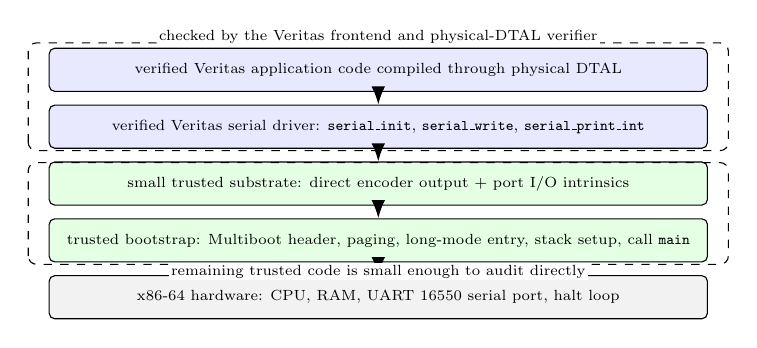
\begin{tikzpicture}[
      scale=0.76,
      transform shape,
      layer/.style={draw, rounded corners=2pt, minimum width=11.0cm, minimum height=0.72cm, align=center, font=\scriptsize},
      trusted/.style={layer, fill=green!10},
      verified/.style={layer, fill=blue!9},
      hardware/.style={layer, fill=gray!10},
      arrow/.style={-Latex, thick}
    ]
    \node[hardware] (hw) at (0,0) {x86-64 hardware: CPU, RAM, UART 16550 serial port, halt loop};
    \node[trusted] (boot) at (0,0.95) {trusted bootstrap: Multiboot header, paging, long-mode entry, stack setup, call \texttt{main}};
    \node[trusted] (rt) at (0,1.9) {small trusted substrate: direct encoder output + port I/O intrinsics};
    \node[verified] (drv) at (0,2.85) {verified Veritas serial driver: \texttt{serial\_init}, \texttt{serial\_write}, \texttt{serial\_print\_int}};
    \node[verified] (app) at (0,3.8) {verified Veritas application code compiled through physical DTAL};

    \draw[arrow] (app) -- (drv);
    \draw[arrow] (drv) -- (rt);
    \draw[arrow] (rt) -- (boot);
    \draw[arrow] (boot) -- (hw);

    \draw[dashed, rounded corners=3pt] (-5.85,2.45) rectangle (5.85,4.25);
    \node[font=\scriptsize, fill=white, inner sep=1pt] at (0,4.36) {checked by the Veritas frontend and physical-DTAL verifier};

    \draw[dashed, rounded corners=3pt] (-5.85,0.55) rectangle (5.85,2.25);
    \node[font=\scriptsize, fill=white, inner sep=1pt] at (0,0.43) {remaining trusted code is small enough to audit directly};
  \end{tikzpicture}
  \caption{Bare-metal Veritas binary structure. The operating system is removed from the trusted computing base; the application and serial driver are compiled from Veritas.}
  \label{fig:bare-metal-unikernel}
\end{figure}

\section{Worked example: binary search}\label{sec:worked-example}
The preceding sections describe each pipeline stage in isolation. This section demonstrates the full pipeline by tracing a \texttt{binary\_search} program, from source to verified DTAL. Binary search features most of the verification and constraint features of Veritas: quantified preconditions, refinement types, loop invariants, array bounds proofs, existential types, branch constraint refinement, and symbolic arithmetic.

\begin{center}
\small
\begin{tabularx}{0.96\linewidth}{@{}p{0.22\linewidth}X@{}}
\toprule
\textbf{Pipeline point} & \textbf{What the example shows} \\
\midrule
Source & The sortedness precondition, loop invariant, and midpoint access state the safety argument. \\
Frontend & The checker turns those facts into SMT obligations, especially the proof that \texttt{arr[mid]} is in bounds. \\
TIR & SSA registers and existential phi constraints keep the loop facts explicit. \\
Physical DTAL & Register allocation and x86-specific expansion rewrite the program before the independent verifier accepts it. \\
\bottomrule
\end{tabularx}
\end{center}

\subsection{Source language}
The source program searches a sorted 10-element array for a target value, returning its index or $-1$ if not found. The proof-relevant fragment is:
\begin{verbatim}
fn binary_search(arr: [int; 10], target: int) -> int
    requires forall i in 0..9 { arr[i] <= arr[i + 1] }
{
    let mut lo: {v: int | v >= 0} = 0;
    let mut hi: int = 9;
    let mut result: int = -1;

    for iter in 0..20
        invariant lo >= 0 && hi < 10
    {
        if lo <= hi {
            let mid: int = lo + (hi - lo) / 2;
            let val: int = arr[mid];
            ... update lo, hi, and result ...
        } else {
            ...
        }
    }

    result
}
\end{verbatim}
Several features are worth highlighting:

\begin{center}
\small
\begin{tabularx}{0.96\textwidth}{>{\raggedright\arraybackslash}p{0.32\textwidth} >{\raggedright\arraybackslash}X}
\toprule
\textbf{Source feature} & \textbf{Role in the proof} \\
\midrule
\texttt{requires forall i in 0..9 \{ arr[i] <= arr[i+1] \}} & Quantified precondition stating sortedness, checked at every call site. \\
\texttt{\{v: int | v >= 0\}} & Master refinement on \texttt{lo}; every assignment must preserve non-negativity. \\
\texttt{invariant lo >= 0 \&\& hi < 10} & Loop invariant bounding both endpoints, checked initially and after the body. \\
\texttt{arr[mid]} & Critical access; the checker must prove $0 \le \mathtt{mid} < 10$. \\
\texttt{for iter in 0..20} & Bounded iteration counter, later preserved as an SSA and DTAL range fact. \\
\bottomrule
\end{tabularx}
\end{center}

\subsection{Frontend type checking}

The type checker discharges three key proof obligations for this function. All are reduced to SMT queries of the form: assert the current context $\phi$, assert $\lnot G$ (the negated goal), and check for unsatisfiability.

\begin{center}
\small
\begin{tabularx}{0.96\textwidth}{>{\raggedright\arraybackslash}p{0.26\textwidth} >{\raggedright\arraybackslash}X}
\toprule
\textbf{Obligation} & \textbf{Why it matters} \\
\midrule
Invariant base case & Shows the loop starts in a state satisfying $\mathtt{lo} \ge 0 \wedge \mathtt{hi} < 10$. \\
Invariant preservation & Shows every branch re-establishes the same invariant before the back edge. \\
Array bounds & Shows the computed midpoint is always a valid index before loading \texttt{arr[mid]}. \\
\bottomrule
\end{tabularx}
\end{center}

The base case follows from the singleton facts $\mathtt{lo}=0$ and $\mathtt{hi}=9$. Preservation is checked branch-by-branch: updates to \texttt{lo} preserve non-negativity, updates to \texttt{hi} preserve the upper bound, and context joining reconciles the branch results. The critical array access occurs under \texttt{lo <= hi}, giving the context:
\[
  \phi = \{\, \mathtt{lo} \ge 0, \;\; \mathtt{hi} < 10, \;\; \mathtt{lo} \le \mathtt{hi}, \;\; \mathtt{mid} = \mathtt{lo} + (\mathtt{hi} - \mathtt{lo}) / 2 \,\}
\]
The SMT oracle proves $0 \le \mathtt{mid} < 10$ from these facts, confirming the bounds proof for \texttt{arr[mid]}.

\subsection{Lowering to TIR (SSA)}
The lowering pass translates the function into a control-flow graph of 13 basic blocks. Figure~\ref{fig:bs-cfg} shows the structure, with blocks grouped by their role in the algorithm.
\begin{figure}[H]
  \centering
  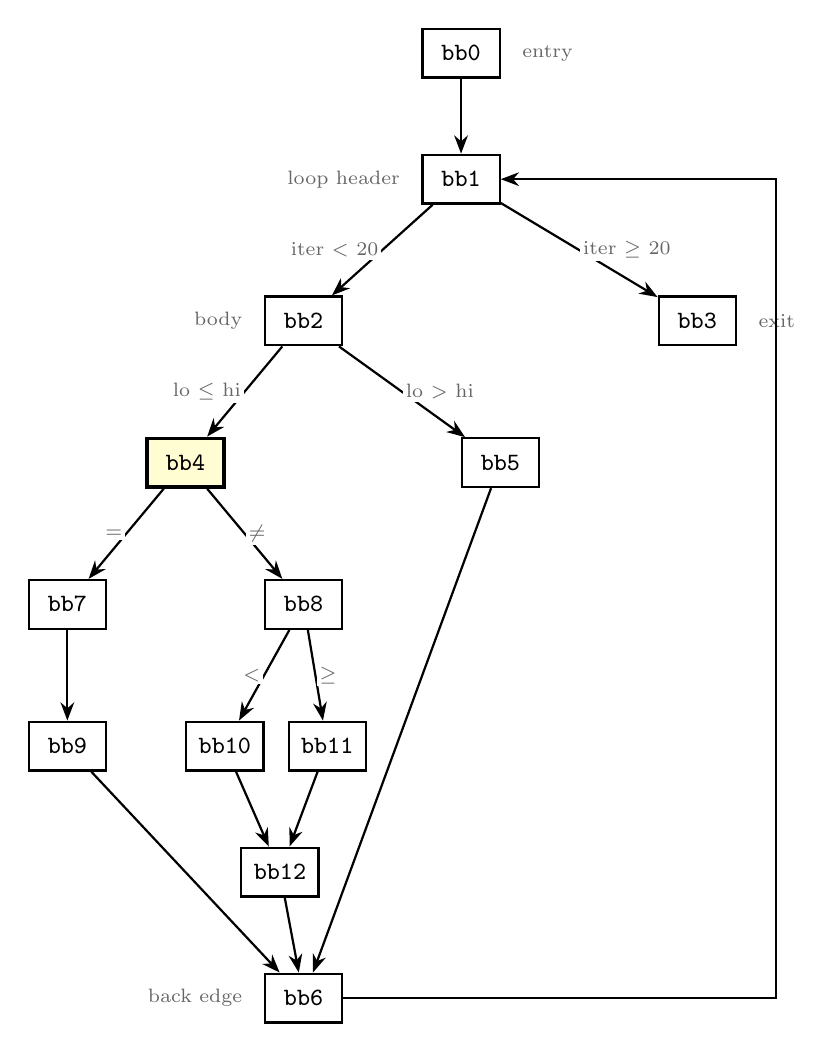
\begin{tikzpicture}[
      scale=1.0, transform shape,
      block/.style={rectangle, draw, thick, text centered,
          minimum height=0.62cm, minimum width=0.98cm,
          font=\small\ttfamily},
      hotblock/.style={rectangle, draw=black, very thick, fill=yellow!18, text centered,
          minimum height=0.62cm, minimum width=0.98cm,
          font=\small\ttfamily},
      arrow/.style={-Stealth, thick},
      lbl/.style={font=\scriptsize, text=black!60},
      elbl/.style={font=\scriptsize, text=black!60, fill=white, inner sep=1pt}
    ]
    \node[block] (bb0) at (0,0) {bb0};
    \node[lbl, right=0.15cm of bb0] {entry};

    \node[block] (bb1) at (0,-1.6) {bb1};
    \node[lbl, left=0.15cm of bb1] {loop header};

    \node[block] (bb2) at (-2,-3.4) {bb2};
    \node[lbl, left=0.15cm of bb2] {body};
    \node[block] (bb3) at (3,-3.4) {bb3};
    \node[lbl, right=0.15cm of bb3] {exit};

    \node[hotblock] (bb4) at (-3.5,-5.2) {bb4};
    \node[block] (bb5) at (0.5,-5.2) {bb5};

    \node[block] (bb7) at (-5,-7.0) {bb7};
    \node[block] (bb8) at (-2,-7.0) {bb8};

    \node[block] (bb9) at (-5,-8.8) {bb9};
    \node[block] (bb10) at (-3,-8.8) {bb10};
    \node[block] (bb11) at (-1.7,-8.8) {bb11};

    \node[block] (bb12) at (-2.3,-10.4) {bb12};

    \node[block] (bb6) at (-2,-12.0) {bb6};
    \node[lbl, left=0.15cm of bb6] {back edge};

    \draw[arrow] (bb0) -- (bb1);
    \draw[arrow] (bb1) -- (bb2) node[elbl, midway, left] {iter $<$ 20};
    \draw[arrow] (bb1) -- (bb3) node[elbl, midway, right] {iter $\ge$ 20};
    \draw[arrow] (bb2) -- (bb4) node[elbl, midway, left] {lo $\le$ hi};
    \draw[arrow] (bb2) -- (bb5) node[elbl, midway, right] {lo $>$ hi};
    \draw[arrow] (bb4) -- (bb7) node[elbl, midway, left] {$=$};
    \draw[arrow] (bb4) -- (bb8) node[elbl, midway, right] {$\ne$};
    \draw[arrow] (bb7) -- (bb9);
    \draw[arrow] (bb8) -- (bb10) node[elbl, midway, left] {$<$};
    \draw[arrow] (bb8) -- (bb11) node[elbl, midway, right] {$\ge$};
    \draw[arrow] (bb10) -- (bb12);
    \draw[arrow] (bb11) -- (bb12);
    \draw[arrow] (bb9) -- (bb6);
    \draw[arrow] (bb12) -- (bb6);
    \draw[arrow] (bb5) -- (bb6);
    \draw[arrow] (bb6.east) -- ++(5.5,0) |- (bb1.east);
  \end{tikzpicture}
  \caption{Control-flow graph of \texttt{binary\_search}. Block bb4 contains the critical array access.}
  \label{fig:bs-cfg}
\end{figure}
Key aspects of the TIR representation:

\begin{center}
\small
\begin{tabularx}{0.96\textwidth}{>{\raggedright\arraybackslash}p{0.27\textwidth} >{\raggedright\arraybackslash}X}
\toprule
\textbf{TIR feature} & \textbf{Effect} \\
\midrule
Loop counter & \texttt{iter} is assigned to virtual register \texttt{v8} with an existential type annotation, capturing $0 \le \texttt{v8} < 20$ without fixing a concrete value. \\
Header phi nodes & Mutable variables (\texttt{lo}, \texttt{hi}, \texttt{result}) become explicit loop-carried registers. Useful refinements, such as \texttt{lo} remaining non-negative, may be preserved existentially. \\
Invariant assertion & The loop invariant appears as an \texttt{AssertConstraint} at the entry of bb2. During code generation this becomes a DTAL \texttt{.assert}, allowing the verifier to re-check it independently. \\
\bottomrule
\end{tabularx}
\end{center}

\subsection{DTAL code generation and verification}
The DTAL output preserves the block structure of the TIR, augmented with entry-state declarations, constraint assumptions, and instruction type annotations.

In the current implementation, \texttt{binary\_search} verifies successfully end-to-end. The first snippet below shows the virtual-register DTAL emitted immediately after code generation. The second shows the corresponding physical DTAL after register allocation and x86-specific expansion, which is the form actually consumed by the final verifier.
\subsubsection{Virtual DTAL: midpoint computation and array access}
\begin{verbatim}
.binary_search_bb4:
    .assume v8 < v7
    .assume (v11 >= 0 && v10 < 10)
    .assume v11 <= v10
    sub v16, v10, v11    : {_synth_0: int | _synth_0 == (hi - lo) }
    mov v17, 2           : int(2)
    div v18, v16, v17    : {_synth_1: int | _synth_1 == ((hi - lo) / 2) }
    add v19, v11, v18    : {_synth_2: int |
                            _synth_2 == (lo + ((hi - lo) / 2)) }
    .assert true
    load v20, [v0 + v19] : int
\end{verbatim}
This virtual DTAL is still close to the source-level reasoning. The branch constraints and invariant have already been translated into register-based assumptions, and the midpoint arithmetic is represented symbolically through the synthesised refinement types on \texttt{v16}, \texttt{v18}, and \texttt{v19}. At this level it is easy to see how the array-bounds proof is carried forward: the load of \texttt{v20} depends on the facts $v11 \ge 0$, $v10 < 10$, and $v11 \le v10$, together with the symbolic definition of the midpoint.
\subsubsection{Physical DTAL: verifier-facing code}
\begin{verbatim}
.binary_search_bb2:
    .assert (r0 >= 0 && r4 < 10)
    cmp r0, r4
    setle lr
    mov r3, lr    : bool
    .type r3: bool
    ble .binary_search_bb4
    jmp .binary_search_bb5
.binary_search_bb4:
    mov lr, r4    : int
    mov r7, r0    : int
    sub lr, lr, r7    : {_synth_0: int | _synth_0 == (hi - lo) }
    mov r10, lr    : {_synth_0: int | _synth_0 == (hi - lo) }
    mov r3, 2    : int(2)
    mov r7, r3    : int
    mov lr, r10    : int
    cqo
    idiv r7
    mov r3, lr    : {_synth_1: int | _synth_1 == ((hi - lo) / 2) }
    mov lr, r0    : int
    mov r7, r3    : int
    add lr, lr, r7    : {_synth_2: int | _synth_2 == (lo + ((hi - lo) / 2)) }
    mov r10, lr    : {_synth_2: int | _synth_2 == (lo + ((hi - lo) / 2)) }
    .assert true
    mov lr, r6    : int
    mov r7, r10   : int
    load lr, [lr + r7]    : int
\end{verbatim}
This is the post-register-allocation DTAL that the final verifier checks. The logical structure is the same as in the virtual DTAL, but the values have been assigned to physical registers and division has been expanded into the x86-64-specific \texttt{cqo}/\texttt{idiv} sequence. The verifier re-derives the types of these arithmetic instructions from their operands, proves that the computed midpoint still satisfies the bounds obligation, and checks state coercion on the loop back edge. This illustrates the key trust-model point: register allocation and target-specific expansion remain untrusted, and the verifier validates their output rather than assuming they are correct.
\subsubsection{Back edge and state coercion}
\begin{verbatim}
.binary_search_bb6:
    mov r3, 1    : int
    mov lr, r9   : int
    mov r7, r3   : int
    add lr, lr, r7    : int
    mov r3, lr   : int
    jmp .binary_search_bb1
\end{verbatim}
At the physical back edge, the loop counter has been allocated to \texttt{r9}. The verifier must show that the exit state of bb6 is compatible with the declared entry state of bb1, including the existential bound on the loop counter and the re-established invariant over the registers holding \texttt{lo} and \texttt{hi}. This is the loop's inductive step in its final, post-register-allocation form.

The worked example is deliberately more detailed than the earlier component descriptions because it shows where the project becomes more than a collection of separate checkers. The frontend proves a source-level array access safe, lowering preserves the relevant facts through SSA, code generation re-expresses them as DTAL assumptions and assertions, register allocation rewrites the program into physical registers, and the verifier still reconstructs enough of the argument to accept the final low-level code. That is the core implementation claim of Veritas in miniature: safety evidence is not only generated at the source level, but survives the path to the executable form at which the untrusted compiler is finally checked.


\chapter{Evaluation}\label{ch:eval}

\section{Evaluation goals and methodology}

This chapter evaluates the core goals of Veritas put forward in the proposal and refined in the requirements analysis (Section~\ref{sec:requirements-anal}).
A central claim of Veritas' architecture is that low-level artefacts can be independently verified while the compiler can be untrusted. Veritas also aimed to support a toolchain for a \emph{systems language}. The evaluation therefore has to assess both the verification story and the ordinary compiler story:

\begin{itemize}
  \item Does DTAL realise the intended trust architecture?
  \item Is the implementation a viable systems-language toolchain?
  \item Is the source language expressive enough for the targeted verification tasks?
  \item Is independent verification practical enough to use?
  \item How much confidence should we have in the verifier?
  \item How much does the architecture reduce the TCB?
\end{itemize}

The evidence used for these questions is deliberately mixed: comparison with Xi and Harper's DTAL, feature-suite coverage, invalid-program rejection, DTAL tampering tests, native code generation, PolyBench-style kernels, wall-clock measurements, solver breakdowns, and a trusted-computing-base analysis for the Linux and bare-metal targets.

The evaluation uses fixed suites rather than ad hoc examples: 28 valid feature programs, 35 invalid source programs, 14 syntax-preserving DTAL tampering cases, and six cross-system comparison tasks. Each suite has a different evidential role. The positive feature suite checks that representative supported programs make it through both the frontend and the independent verifier. The negative suite checks that unsafe source programs are rejected rather than accidentally accepted. The DTAL tampering corpus starts from valid compiled DTAL and mutates the low-level program, directly testing the untrusted-compiler story. The cross-system suite gives a small normalised comparison against established verification tools.

Timing results use two measurement layers. Internal metrics from \texttt{veritas --bench} separate source-to-DTAL compilation, explicit DTAL verification, and SMT time; \texttt{hyperfine} wall-clock timings include process startup and native-output generation. Runtime correctness is checked using exact outputs or deterministic checksums, not successful termination alone. This distinction is important because a verifier can appear cheap or expensive depending on whether one measures only the checking phase, the full command invocation, or the generated program's runtime behaviour. The chapter therefore treats these as separate claims rather than folding them into one performance number.

\section{DTAL design and implementation}\label{sec:dtal-eval}

In the Veritas architecture, the target DTAL must be expressive enough to enable verification of the required safety properties. The evaluation considers to what extent the DTAL implementation supports the intended trust architecture.

\subsection{Relationship to Xi and Harper's DTAL}

Veritas is inspired directly by Xi and Harper's DTAL and preserves many of its central features and ideas most relevant for independent low-level verification:

\begin{center}
\small
\begin{tabularx}{0.96\textwidth}{>{\raggedright\arraybackslash}p{0.32\textwidth} >{\raggedright\arraybackslash}X}
\toprule
\textbf{DTAL mechanism} & \textbf{Safety role} \\
\midrule
Dependent block or label state & Supports control-flow safety by ensuring that jumps and joins are only valid when the incoming machine state matches the target's expected typing context. \\
Singleton integer typing & Supports arithmetic and indexing safety, since later instructions can rely on symbolic facts when proving side conditions. \\
Size-indexed arrays & Supports memory safety by making out-of-bounds reads and writes statically checkable. \\
Typed stack discipline & Supports structural safety by preventing ill-typed stack use across calls, returns, and local temporaries. \\
Proof-relevant typed memory access & Supports static memory-safety guarantees such as array-bound-check elimination. \\
\bottomrule
\end{tabularx}
\end{center}

Veritas narrows Xi and Harper's design in some directions. It does not expose their full tuple and allocation primitives, broad existential dependent types, or sum and tag reasoning. Instead, it focuses on the low-level facts needed for fixed-size arrays, arithmetic side conditions, contracts, and borrow-aware compilation. This sacrifices theoretical generality in exchange for automation and a verification model that fits the rest of the toolchain.

The most important continuity with Xi and Harper's DTAL lies in the independent low-level verification model. The Veritas version of the copy-loop pattern from Section~\ref{sec:dtal-background} preserves the same basic idea of typed labels and register-indexed array access, although the surface syntax is adapted to its implementation:

\begin{quote}
  \begin{verbatim}
.entry {v0: int}
.assume (v0 >= 0 && v0 < 4)
add v9, v0, v8    : {_synth_0: int | _synth_0 == (i + 1) }
.assert true
load v10, [v1 + v9]    : int(7)
\end{verbatim}
\end{quote}

The low-level program records sufficient information for the verifier to justify array access from the surrounding type and constraint context rather than relying on a dynamic bounds check.

\subsection{Extensions and deviations}


Veritas preserves the same basic typed memory access idea, but also extends it with explicit refinement-carrying annotations that originate in source-level proof obligations, for example:
\begin{quote}
  \begin{verbatim}
div v2, v0, v1    : {_synth_0: int | _synth_0 == (a / b) }
load v10, [v1 + v9]    : int(7)
  \end{verbatim}
\end{quote}
These carried obligations are re-checked by the verifier against the low-level code. This provides a broader source-to-low-level continuity for the particular fragment Veritas supports, including not just bounds facts but also contract-style and borrow-related safety obligations. Preserving additional proof-relevant annotations does increase the surface on which an untrusted compiler can introduce inconsistencies, and therefore may increase the risk of false rejection, but it does not expand the acceptance surface or weaken verification guarantees.

Another extension is the introduction of explicit ownership and borrow-aware operations.
This extension pushes alias-control properties below the frontend where the relevant low-level operations are represented and re-checked in DTAL. This is a significant divergence from Xi and Harper's DTAL in order to serve a systems-language setting.

\begin{quote}
  \begin{verbatim}
alias_borrow v3, v1    : &[int(7); 1]
load v5, [v3 + v4]     : int
borrow_end v3          : &[int(7); 1]
  \end{verbatim}
\end{quote}

In this example, the creation, use, and termination of the borrowed view is represented explicitly in DTAL, which allows the verifier to check that the access occurs through a live borrow and that the borrow is ended consistently with the source-language ownership discipline.

Because verification happens after physical register allocation, Veritas defines a `physical DTAL' with explicit scratch-register use, spills, prologues/epilogues, and instruction expansions. Xi and Harper's DTAL is closest to Veritas' virtual DTAL: its semantics are given over an abstract machine, and register allocation and spilling are explicitly not modelled. The difference is visible in instructions such as:

\begin{quote}
  \begin{verbatim}
mov lr, r1    : int
cqo
idiv r7
mov r0, lr    : int
\end{verbatim}
\end{quote}

or in explicit stack and calling-convention machinery such as
\texttt{spill\_store}, \texttt{spill\_load}, \texttt{.prologue}, and
\texttt{.epilogue}.
The main tradeoff is low-level complexity. Physical DTAL exposes register assignments, spill slots, calling-convention details, and instruction expansion that are absent from the source language. This makes the representation less elegant than an idealised typed assembly and increases the burden on the verifier. However, it also makes register allocation and instruction expansion part of the untrusted compiler, which is more useful for the project's trust model.




\section{Veritas as a systems-language toolchain}\label{sec:veritas-sys-eval}

This section evaluates Veritas as a systems-language toolchain. The project applies the trust architecture in a systems-oriented setting, where memory safety has to coexist with imperative control flow, mutable state, references, predictable data representation, and native code generation. Veritas is far less mature than C or Rust in language breadth, tooling, and ecosystem, so the relevant question is narrower: within the intended fragment, does it behave like a plausible systems-language design that could be built on further?


\subsection{Systems-language feature comparison}

Compared with C and Rust, Veritas occupies an intermediate position. Like both languages, it supports first-order functions, mutable local state, fixed-size arrays, loop-based imperative control flow, and native-code compilation. Like Rust, it has an ownership- and borrow-aware safety story rather than relying purely on unrestricted memory manipulation. Unlike both, its design is centred around carrying verification-relevant information through the compilation pipeline. This makes Veritas less general-purpose than C or Rust, but gives it a stronger explicit safety and trust architecture within its supported fragment.


\begin{table}[H]
  \centering
  \small
  \begin{tabularx}{0.96\textwidth}{>{\raggedright\arraybackslash}X c c >{\raggedright\arraybackslash}p{0.22\textwidth}}
    \hline
    \textbf{Feature}                            & \textbf{C} & \textbf{Rust} & \textbf{Veritas}                      \\
    \hline
    Mutable local state                         & \checkmark & \checkmark    & \checkmark                            \\
    Fixed-size arrays                           & \checkmark & \checkmark    & \checkmark                            \\
    Structured loop control flow                & \checkmark & \checkmark    & \checkmark                            \\
    Native-code compilation                     & \checkmark & \checkmark    & \checkmark                            \\
    Built-in ownership discipline               &            & \checkmark    & \checkmark                            \\
    Refinement/contracts/invariants             &            &               & \checkmark                            \\
    Independent low-level verifier              &            &               & \checkmark                            \\
    User-defined structs / algebraic data types & \checkmark & \checkmark    & arrays / refs only                    \\
    General heap allocation model               & \checkmark & \checkmark    & restricted \texttt{alloca} only       \\
    General unrestricted pointers               & \checkmark & \checkmark    &                                       \\
    Basic I/O and runtime interaction           & \checkmark & \checkmark    & partial                               \\
    Mature module / package ecosystem           & \checkmark & \checkmark    &                                       \\
    FFI / systems-library integration story     & \checkmark & \checkmark    & minimal                               \\
    Heap-heavy general systems idioms           & \checkmark & \checkmark    & array / ref kernels only              \\
    Concurrency model in current fragment       & \checkmark & \checkmark    &                                       \\
    \hline
  \end{tabularx}

  \caption{High-level comparison of Veritas with C and Rust as systems-language
    toolchains.}
  \label{tab:systems-language-comparison}
\end{table}

The shared features are enough for the low-level kernels and array-oriented routines used throughout the evaluation. The missing features still limit its generality, but within a narrower fragment centred on structured imperative code with strong safety tracking, Veritas exhibits recognisably systems-language behaviour while offering a more explicit verification and trust model than conventional toolchains.

\subsection{Compiler functional correctness}

The architecture treats the compiler as untrusted, but it should still behave like a plausible toolchain. Since the compiler is not formally proved correct, this part of the evaluation is empirical and corpus-based: it asks whether generated binaries agree with the intended semantics on fixed suites.

\begin{center}
\small
\begin{tabularx}{0.96\textwidth}{>{\raggedright\arraybackslash}p{0.22\textwidth} >{\raggedright\arraybackslash}p{0.18\textwidth} >{\raggedright\arraybackslash}X}
\toprule
\textbf{Suite} & \textbf{Result} & \textbf{Role in the argument} \\
\midrule
\texttt{feature\_suite} & 28 / 28 pass & Local correctness corpus for arrays, mutable state, borrowing, contracts, invariants, quantifiers, safe division, and overflow-aware arithmetic. \\
PolyBench-style kernels & 7 / 7 pass & External check on recognised array- and loop-dominated workloads, validated by stable checksums against C baselines. \\
\bottomrule
\end{tabularx}
\end{center}

The feature suite checks the constructs and proof obligations Veritas was built to support. The PolyBench-style suite is more objective: PolyBench/C is widely used for compiler and program-transformation evaluation, and its kernels contain regular control flow, affine array indexing, and deterministic numeric behaviour.

\begin{table}[h]
  \centering
  \small
  \begin{tabularx}{0.96\textwidth}{>{\raggedright\arraybackslash}p{0.17\textwidth} >{\raggedright\arraybackslash}p{0.18\textwidth} >{\raggedright\arraybackslash}X}
    \hline
    \textbf{Kernel} & \textbf{\texttt{MEDIUM} params} & \textbf{Why it is included} \\
    \hline
    Floyd--Warshall & \texttt{N=500} & Dynamic programming over a weighted graph matrix; stresses nested loops, fixed-size 2D arrays, arithmetic updates, and indexed mutation. \\
    Jacobi-1D       & \texttt{N=400}, \texttt{T=100} & Iterative stencil update over repeated time steps; stresses affine indexing and arithmetic recurrences. \\
    Jacobi-2D       & \texttt{N=250}, \texttt{T=100} & Two-dimensional stencil computation; stresses neighbourhood indexing over fixed-size arrays. \\
    Seidel-2D       & \texttt{N=400}, \texttt{T=100} & In-place smoothing stencil; stresses array mutation and affine neighbour access. \\
    MVT             & \texttt{N=400} & Matrix-vector and transposed-matrix-vector multiplication; stresses regular matrix/vector indexing. \\
    ATAX            & \texttt{M=390}, \texttt{N=410} & Matrix-transpose-times-vector computation; stresses multiple loop phases and intermediate accumulation. \\
    GESUMMV         & \texttt{N=250} & Weighted sum of two matrix-vector products; stresses linear-algebra style arithmetic and nested loops. \\
    \hline
  \end{tabularx}
  \caption{PolyBench-style kernels used in the Veritas evaluation, with their
    fixed \texttt{MEDIUM}-class parameters and the main compiler behaviours
    they exercise.}
  \label{tab:polybench-kernels}
\end{table}

Table~\ref{tab:polybench-kernels} gives a spread across dynamic-programming, stencil, and matrix/vector-style computations. These are appropriate for Veritas because the language and verifier are strongest on fixed-size arrays, structured imperative loops, arithmetic side conditions, and deterministic computation over statically bounded data. All seven kernels pass their defined semantic checks.

While these results do not amount to full compiler correctness in the CompCert sense, nor does it imply that every future program in the Veritas fragment will automatically enjoy the same guarantee, it supports a strong suite-bounded claim: for the representative local feature corpus and the committed external kernel corpus, the delivered compiler both preserves verifier-relevant structure and produces binaries whose observed behaviour matches the intended semantics.

\subsection{Compiler and runtime practicality}

Practicality is evaluated at two levels: compilation cost and runtime behaviour of the generated binaries. The curated \texttt{feature\_suite} provides a useful summary of compiler throughput.

\begin{figure}[H]
  \centering
  \includegraphics[width=0.8\textwidth]{figures/chapter4_feature_suite_compile_cost.png}
  \caption{Compile-cost structure across the curated feature suite.}
  \label{fig:feature-suite-compile-cost}
\end{figure}


Figure~\ref{fig:feature-suite-compile-cost} makes the dominant cost pattern clear: binary-search, array-proof, and quantifier-heavy programs are the most expensive to compile, and a significant share of that cost is solver time. Simpler arithmetic- and borrow-oriented cases remain much cheaper.

The external PolyBench-style kernels provide a second view on larger loop- and array-heavy programs. Here compile time is dominated more strongly by frontend SMT work, because the kernels repeatedly exercise affine array indexing, nested loops, and arithmetic side conditions. Figure~\ref{fig:polybench-compile-cost} shows that the fastest kernel still compiles in under half a second, while the most expensive kernels take tens of seconds and are again dominated by solver-heavy proof structure rather than by raw source size alone.

\begin{figure}[H]
  \centering
  \includegraphics[width=0.92\textwidth]{figures/chapter4_polybench_compile_cost.png}
  \caption{Compile-cost structure across the translated PolyBench-style kernel suite.}
  \label{fig:polybench-compile-cost}
\end{figure}


Runtime practicality is evaluated using the same PolyBench-style kernel set to ask whether compiled verified kernels remain plausible executable programs. All included kernels pass semantic validation, and runtime performance relative to GCC varies substantially by workload.

\begin{figure}[H]
  \centering
  \includegraphics[width=0.92\textwidth]{figures/chapter4_polybench_runtime_absolute.png}
  \caption{Absolute runtime for the committed \texttt{MEDIUM}-class PolyBench-style suite. The figure compares Veritas against GCC \texttt{-O3} and checked C \texttt{-O3}; all plotted kernels passed checksum-based semantic validation before timing results were accepted.}
  \label{fig:polybench-runtime-absolute}
\end{figure}

The results in Figure~\ref{fig:polybench-runtime-absolute} show a mixed pattern rather than a uniform slowdown. On the \texttt{MEDIUM}-class PolyBench suite, MVT and GESUMMV are relatively close to the GCC \texttt{-O3} baseline, at roughly 1.55$\times$ and 1.10$\times$ respectively, while Floyd--Warshall, Jacobi-2D, and Seidel-2D are slower by roughly 3.3--5.9$\times$. This shows that runtime performance depends strongly on workload shape rather than following a single fixed overhead pattern.

To test whether the fixed-suite results were stable beyond one benchmark size, a follow-up size sweep was run on the more stable kernels. Each kernel was timed for Veritas, GCC \texttt{-O3}, and a checked C \texttt{-O3} baseline, where `checked C' denotes the manually instrumented variant with explicit dynamic array-bounds checks.

\begin{figure}[H]
  \centering
  \includegraphics[width=0.96\textwidth]{figures/chapter4_polybench_scaling_absolute.png}
  \caption{Runtime scaling for the chapter-facing PolyBench follow-up sweep. These size sweeps are anchored around the \texttt{MEDIUM}-class kernel sizes and compare Veritas with GCC \texttt{-O3} and checked C \texttt{-O3}.}
  \label{fig:polybench-scaling-absolute}
\end{figure}

Figure~\ref{fig:polybench-scaling-absolute} supports the same interpretation as the fixed-size suite. Stencil-style and dynamic-programming kernels remain slower than both C baselines, while the lighter matrix/vector kernels stay much closer. Veritas therefore does not incur one uniform slowdown on array-heavy programs; the relative runtime cost depends strongly on the computational pattern being compiled. The generated code is executable, semantically validated, and often within a small constant factor of compiled C on the tested kernels, while also participating in a verification pipeline that C itself does not provide.

Binary size is a supporting practicality metric. The larger loop-heavy kernels compile to small freestanding Veritas binaries, typically around 1.4--2.4\,KB. Veritas code is larger than GCC's \texttt{.text} section across the suite, but not by an order of magnitude, which is consistent with a research backend that prioritises verifier-visible structure over code density.

\section{Source language expressiveness for verification}\label{sec:source-lang-eval}

This section focuses on the source language as a verification-oriented language. It evaluates what kinds of properties it can express in practice, how that compares with related verification languages, and why the source-level expressiveness story is different in Veritas because the resulting proof-relevant information is preserved into DTAL rather than erased after frontend checking.

\subsection{Properties expressible in Veritas}

Within the supported fragment, Veritas can express contracts, loop invariants, bounded quantified properties, array-bounds and arithmetic safety conditions, sortedness-style properties, and borrowing constraints. It is not yet a mature verification ecosystem, but it is expressive enough for the dissertation's array-heavy programs.

\begin{center}
\small
\begin{tabularx}{0.96\textwidth}{>{\raggedright\arraybackslash}p{0.30\textwidth} >{\raggedright\arraybackslash}X}
\toprule
\textbf{Expressive strength} & \textbf{Current limit} \\
\midrule
Sorted arrays, bounded indices, loop invariants, arithmetic side conditions, postconditions, and ownership constraints. & No rich user-defined algebraic datatypes, no mature ghost-state discipline, no general heap model, and no interactive proof layer. \\
\bottomrule
\end{tabularx}
\end{center}

The strongest examples align with the language's first-order, loop-based style. These are not toy properties: they are exactly the obligations that make ordinary systems code fragile when written in an unchecked language. The implemented language is deliberately narrower than Dafny, Verus, or Liquid Haskell as a general verification environment. Its distinct contribution is that the properties it can express are carried into the compiled low-level representation and checked there independently.

\subsection{Comparison with verification-oriented languages}

The most appropriate comparison points are Dafny, Liquid Haskell, Verus, and ATS. Dafny is the closest imperative SMT-backed verifier, Liquid Haskell is the closest refinement-type automation baseline, Verus is the most relevant modern systems-language verification comparison, and ATS is the clearest historical predecessor for Veritas' broader goals.


\begin{table}[h]
  \centering
  \scriptsize
  \begin{tabular}{@{}p{0.43\textwidth} c c c c c@{}}
    \hline
    \textbf{Safety property / constraint class}         & \textbf{Veritas} & \textbf{Dafny} & \textbf{LH} & \textbf{Verus} & \textbf{ATS} \\
    \hline
    Array bounds safety                                 & \checkmark       & \checkmark     & partial                 & \checkmark     & \checkmark   \\
    Division-by-zero safety                             & \checkmark       & \checkmark     & \checkmark              & \checkmark     & \checkmark   \\
    Overflow / arithmetic side-condition reasoning      & \checkmark       & partial        & partial                 & \checkmark     & \checkmark   \\
    Preconditions and postconditions                    & \checkmark       & \checkmark     & \checkmark              & \checkmark     & \checkmark   \\
    Loop invariant reasoning                            & \checkmark       & \checkmark     & partial                 & \checkmark     & partial      \\
    Quantified specifications                           & \checkmark       & \checkmark     & partial                 & \checkmark     & partial      \\
    Sortedness / predicate-rich functional properties   & \checkmark       & \checkmark     & \checkmark              & \checkmark     & \checkmark   \\
    Ownership / aliasing discipline                     & \checkmark       & --             & --                      & \checkmark     & partial      \\
    Heap-allocated linked data structure invariants     & --               & \checkmark     & \checkmark              & partial        & partial      \\
    Recursive structural functional correctness proofs  & --               & \checkmark     & \checkmark              & \checkmark     & \checkmark   \\
    Concurrency / data-race freedom properties          & --               & --             & --                      & \checkmark     & --           \\
    Ghost-state-heavy protocol reasoning                & partial          & \checkmark     & partial                 & \checkmark     & \checkmark   \\
    Information-flow / noninterference-style properties & --               & partial        & partial                 & partial        & partial      \\
    Low-level preservation of checked constraints       & \checkmark       & --             & --                      & --             & --           \\
    Independent checking of compiled artefact           & \checkmark       & --             & --                      & --             & --           \\
    \hline
  \end{tabular}
  \caption{Comparison of the main safety properties and specification classes relevant to this dissertation. ``Partial'' indicates that the property is expressible, but less naturally or less directly in the style of programs considered here. LH abbreviates Liquid Haskell.}
  \label{tab:verification-safety-properties}
\end{table}


Table~\ref{tab:verification-safety-properties} makes the current limits of Veritas clearer: the implemented fragment is strong on array-heavy safety properties, arithmetic side conditions, contracts, and borrow-aware reasoning, but weak on heap-shaped invariants, recursive proof patterns, concurrency properties, and more protocol-oriented ghost-state verification. Where Veritas starts to diverge is in its ability to preserve the checked constraints in the fragments it does support below the source language.



The cross-system comparison suite contains six normalised tasks: preconditioned safe division, bounded array access with an offset, array initialisation with a loop invariant, binary search over a sorted collection, returning the head of a sorted array, and overflow-safe midpoint arithmetic. The suite is normalised by verified property: Dafny uses heap arrays, Veritas and Verus use fixed-size arrays naturally, and Liquid Haskell uses a more functional representation.

\begin{figure}[H]
  \centering
  \includegraphics[width=\linewidth]{figures/chapter4_annotation_burden.png}
  \caption{Annotation-to-code ratios across the normalised six-task
    cross-system comparison suite.}
  \label{fig:cross-system-annotation-burden}
\end{figure}

Within this small suite, Figure~\ref{fig:cross-system-annotation-burden} shows Veritas is competitive on annotation burden and is particularly light on the loop- and search-heavy tasks.



\section{Verification cost and performance}\label{sec:verification-perf}

This section asks how expensive those checks are, where the cost appears, and how Veritas should be compared with source-level verification systems that do not perform an explicit low-level re-checking stage.

\subsection{Veritas verification cost breakdown}

The first layer of cost evidence comes from the curated feature suite. These results separate source-to-DTAL compilation cost from the explicit DTAL verification stage.

\begin{center}
\small
\begin{tabularx}{0.88\textwidth}{>{\raggedright\arraybackslash}p{0.36\textwidth} r >{\raggedright\arraybackslash}X}
\toprule
\textbf{Metric} & \textbf{Mean} & \textbf{Worst case} \\
\midrule
Source-to-DTAL compilation & 27.110\,ms & \texttt{binary\_search}, 163.817\,ms \\
Explicit DTAL verification & 9.116\,ms & \texttt{binary\_search}, 55.209\,ms \\
Frontend SMT time & 13.097\,ms & Proof-heavy programs dominate \\
Verifier SMT time & 8.737\,ms & Proof-heavy programs dominate \\
\bottomrule
\end{tabularx}
\end{center}

For the current supported fragment, the mean explicit verifier cost is materially smaller than the mean frontend source-to-DTAL cost. The most expensive programs are also the proof-heavy ones: binary search mixes loop invariants, symbolic arithmetic, and sortedness-oriented reasoning, while simpler contract and borrow examples remain much cheaper.

The second layer of cost evidence comes from the verification-stress suite, a subset of the feature suite that acts as a proof-oriented stress suite of obligation-heavy programs.


\begin{table}[h]
  \centering
  \small
  \begin{tabular}{l r r r}
    \hline
    \textbf{Program}              & \textbf{Compile only (s)} & \textbf{Compile + verify (s)} & \textbf{Overhead ratio} \\
    \hline
    \texttt{array\_init}          & 0.0648                    & 0.2280                        & 3.521x                  \\
    \texttt{array\_assignment}    & 0.0890                    & 0.1089                        & 1.223x                  \\
    \texttt{quantifier\_showcase} & 0.1607                    & 0.1835                        & 1.142x                  \\
    \texttt{binary\_search}       & 0.2473                    & 0.2516                        & 1.017x                  \\
    \texttt{bubble\_sort}         & 0.0848                    & 0.1175                        & 1.385x                  \\
    \texttt{sortedness}           & 0.0283                    & 0.0394                        & 1.393x                  \\
    \hline
  \end{tabular}
  \caption{End-to-end wall-clock overhead of explicit DTAL verification on the
    verification-stress suite.}
  \label{tab:verification-stress-overheads}
\end{table}

Table~\ref{tab:verification-stress-overheads} shows that the cost of the independent verifier is highly program-dependent. \texttt{array\_init} is the clearest outlier, with a 3.521$\times$ overhead ratio, because it generates a particularly obligation-heavy array initialisation pattern.

\subsection{Cross-system verification-cost comparison}

The comparison suite supports a small empirical contrast with Dafny, Liquid Haskell, and Verus on six normalised tasks: safe division, bounded array access with an offset, array initialisation with a loop invariant, binary search, sorted-head extraction, and overflow-safe midpoint arithmetic. Repeated wall-clock timings were collected locally for Veritas in both \texttt{compile\_only} and \texttt{compile\_plus\_verify} modes, and for the other systems using their normal source-level verification commands.

\begin{figure}[H]
  \centering
  \includegraphics[width=0.86\linewidth]{figures/chapter4_comparison_suite_wallclock.png}
  \caption{Grouped wall-clock timings for the normalised six-task
    cross-system comparison suite. Bars show mean time and error bars show one
    standard deviation. The Veritas results were refreshed at 100 runs with 10
    warmups; the external-system results use the corresponding repeated local
    verification-command measurements.}
  \label{fig:comparison-suite-wallclock}
\end{figure}

Figure~\ref{fig:comparison-suite-wallclock} shows the resulting wall-clock times. Veritas averages around 0.038\,s in \texttt{compile\_only} mode and 0.047\,s in \texttt{compile\_plus\_verify} mode over 100 runs with 10 warmups. Dafny averages $\sim$1.016\,s, Liquid Haskell $\sim$1.227\,s, and Verus $\sim$0.488\,s, with \texttt{binary\_search} again the most expensive case for all systems. The comparison should not be read as a general speed ranking: Veritas verifies a deliberately smaller fragment, while the other systems run their full source-level verification pipelines. Its relevance is that the extra low-level checking stage remains small on the normalised tasks.

A key distinction is that Veritas incurs two separable verification costs, at the source and DTAL level, whereas most related systems primarily incur one.
The frontend-only view, approximated by \texttt{compile\_ms} and the frontend SMT metrics, is the fairest comparison point against source-level verification systems. The end-to-end view, measured by \texttt{compile\_plus\_verify} wall-clock timings and \texttt{verify\_ms}, is the relevant measure for the trust architecture.
The other systems report only source-level verification time because they do not attempt an analogous independently checkable low-level stage.

\section{Verifier functional correctness and reliability}\label{sec:verifier-correctness}

This section evaluates the verifier itself as an independent checking mechanism. The claim is not that the verifier has been proved correct in a formal metatheoretic sense, but that it behaves reliably in practice.

\begin{center}
\small
\begin{tabularx}{0.96\textwidth}{>{\raggedright\arraybackslash}p{0.22\textwidth} >{\raggedright\arraybackslash}p{0.20\textwidth} >{\raggedright\arraybackslash}X}
\toprule
\textbf{Evidence} & \textbf{Result} & \textbf{What it supports} \\
\midrule
\texttt{feature\_suite} & 28 / 28 accepted & Frontend compiler and independent physical-DTAL verifier agree on representative valid programs. \\
\texttt{negative\_suite} & 35 / 35 rejected & Source-level checking rejects representative unsafe programs across the main error modes (Table~\ref{tab:negative-suite-summary}). \\
\texttt{dtal\_tampering} & 14 / 14 rejected & The low-level verifier rejects representative corruptions introduced after source compilation. \\
\bottomrule
\end{tabularx}
\end{center}

The first two rows establish that the frontend and verifier agree on the supported source fragment: representative valid programs compile and verify, while representative unsafe programs are rejected before code generation. The third row is stronger evidence for Veritas' distinctive claim, because it checks what happens after a valid source program has already passed the frontend and an untrusted later phase corrupts the low-level artefact.

\subsection{Rejection of tampered DTAL}

The most distinctive reliability evidence is the DTAL tampering corpus, since it tests the trust boundary directly rather than only the source language. A valid source program is compiled to DTAL, the baseline DTAL is verified successfully, and then a small syntax-preserving mutation is applied to the low-level program. The verifier is expected to reject the tampered DTAL.

The current corpus contains 14 cases spanning return-signature mismatches, strengthened preconditions, contradictory assertions, positive and negative out-of-bounds accesses, arithmetic overflow, use-after-drop, ownership duplication, mutable-aliasing violations, and entry state or signature mismatches. The mutations are deliberately small, because this is the shape a backend bug can take.

\begin{center}
\small
\begin{tabularx}{0.96\linewidth}{@{}p{0.24\linewidth}X@{}}
\toprule
\textbf{Tamper} & \textbf{Why the verifier rejects it} \\
\midrule
\texttt{.returns int} changed to \texttt{.returns bool} & The return register's re-derived type no longer satisfies the declared function contract. \\
Safe array index changed to an out-of-bounds constant & The verifier can no longer prove the low-level load or store index is inside the array extent. \\
Duplicating move inserted after a live borrow & The ownership state now contains two usable aliases to a resource that should remain linear. \\
\bottomrule
\end{tabularx}
\end{center}

These mutations are rejected at exactly the point where an untrusted backend would otherwise be relied on.

This evidence shows that representative low-level corruptions are rejected even when the original source program was valid.


\section{Trust architecture and trusted computing base}\label{sec:tcb-eval}

This section returns to the dissertation's architectural claim: Veritas should not only verify useful programs, but do so with a smaller and more explicit trust boundary than a source-level-only verification pipeline. The main question here is what remains trusted once independent physical-DTAL verification is in place.

\subsection{Trusted computing base analysis}
In the current design, the frontend, lowering pipeline, register allocator, physical allocation pass, and most backend logic are intentionally untrusted: bugs in those components should be exposed as verification failure. Table~\ref{tab:tcb-summary} separates the measured verifier-side Rust core from the small trusted artefacts that remain below it on the Linux and bare-metal targets.

\begin{table}[ht]
  \centering
  \small
  \begin{tabular}{l l l c c}
    \hline
    \textbf{Trusted component} & \textbf{Form}         & \textbf{Size}             & \textbf{Linux} & \textbf{Unikernel} \\
    \hline
    DTAL verifier core         & Rust LOC              & 7372 / 34581 (21.3\%)     & \checkmark     & \checkmark         \\
    Direct encoder             & Rust LOC              & 328                       & \checkmark     & \checkmark         \\
    x86 instruction encoder    & Rust LOC              & 792                       & \checkmark     & \checkmark         \\
    Z3 solver                  & external tool         & large external dependency & \checkmark     & \checkmark         \\
    Runtime blob               & machine code          & 418 bytes                 & \checkmark     & --                 \\
    Multiboot bootstrap        & machine code          & 206 bytes                 & --             & \checkmark         \\
    Host OS / kernel           & execution environment & large external dependency & \checkmark     & --                 \\
    \hline
  \end{tabular}
  \caption{Decomposed trust architecture for the current Veritas
    implementation. The verifier-side Rust LOC measurement captures the main
    trusted implementation core; the remaining rows distinguish the additional
    trusted artefacts for Linux and bare-metal targets.}
  \label{tab:tcb-summary}
\end{table}

The verifier-side Rust core is \num{7372} lines out of \num{34581} non-test Rust lines, or 21.3\% of the counted implementation.
While this remains a substantial audit target in absolute terms, it does mean that most of the compiler remains outside the trusted path. The decomposition also shows how I/O changes the trust model. On Linux, adding I/O adds a small trusted runtime blob and its typed interface, while the verifier still re-checks all call sites independently. On the bare-metal target, that runtime layer is largely replaced by DTAL-verified Veritas code, leaving mainly the encoder and the 206-byte bootstrap beneath the verifier.

The important comparison is not only the number of trusted lines, but which lines they are. A conventional source-level verification pipeline still trusts later compilation and code generation to preserve the source-level result. A fully verified compiler instead tries to prove that the whole translation is semantics-preserving, but that proof is a large artefact in its own right. Veritas takes a more modest route: it trusts an independent checker for a lower-level language and a small encoder beneath it. That does not remove all trust, since Z3, the verifier implementation, and the final encoder still matter, but it gives a concrete and inspectable boundary around the code responsible for accepting executable artefacts.

\section{Threats to validity and limitations}

The results support the dissertation's main claims, but only for the current fragment and benchmark policy.

\begin{center}
\small
\begin{tabularx}{0.96\textwidth}{>{\raggedright\arraybackslash}p{0.28\textwidth} >{\raggedright\arraybackslash}X}
\toprule
\textbf{Threat} & \textbf{Scope of the claim} \\
\midrule
Benchmark coverage & Strongest evidence is for arrays, local mutation, contracts, loop invariants, quantifiers, borrowing, and structured numeric kernels. It is not evidence for heap-heavy data structures, arbitrary pointer manipulation, concurrency, or large module ecosystems. \\
Cross-system comparison & Dafny, Liquid Haskell, Verus, and Veritas differ in host language, proof style, and what counts as a natural encoding of a property. Veritas also pays both source-level checking cost and DTAL-level checking cost. \\
Verifier assurance & The feature suite, negative suite, and tampering corpus show coherent behaviour on the supported fragment, but do not prove verifier soundness or completeness. \\
\bottomrule
\end{tabularx}
\end{center}

\section{Summary against project objectives}

\componentblock{Source safety obligations are expressible}{Contracts, invariants, quantifiers, arrays, and borrowing examples are supported, within the current fragment. The remaining limitation is language coverage rather than the shape of the verification architecture.}
\componentblock{Safety evidence survives lowering}{TAST, TIR, DTAL annotations, and the binary-search trace show the relevant facts moving through the compiler rather than being erased. This is the key type-preservation evidence: the compiler emits proof-relevant structure that a later checker can inspect.}
\componentblock{Low-level output is checked independently}{\texttt{--verify-dtal}, physical-DTAL verification, and agreement on 28 / 28 valid programs show that the verifier can check compiled artefacts without using the source compiler. The trusted base still includes Z3, the verifier implementation, and the final encoder, but not the optimisation or lowering passes.}
\componentblock{Executable output is produced}{The toolchain emits Linux ELF binaries, uses a small runtime, supports a bare-metal target, and runs the PolyBench-style kernels. It is therefore an executable compiler prototype rather than only a formal model, although it is not a GCC-level optimiser.}
\componentblock{Compiler bugs can be exposed after compilation}{The DTAL tampering corpus rejects 14 / 14 representative low-level corruptions. This demonstrates the intended failure mode: compiler output that no longer justifies its safety annotations is rejected after compilation, before execution. It is empirical evidence rather than a machine-checked proof of verifier correctness.}

The evaluation therefore supports the dissertation's central claim: Veritas is more than a source-level refinement prototype. It is a working type-preserving compilation pipeline in which proof-relevant information is preserved to a low-level representation and independently re-checked there.

The core objectives are met: Veritas implements a DTAL-inspired trust architecture, verifies compiled low-level artefacts independently, supports a non-trivial source fragment, produces executable code, and gives a meaningful external practicality story through the translated PolyBench-style kernels. The partial objectives are scope-related rather than architectural: runtime performance and code quality are not yet competitive with mature systems compilers, and the supported fragment remains narrower than a mature systems language or general-purpose verification platform.

The strongest overall conclusion is architectural. Veritas occupies a distinct and well-evidenced point between source-level verification tools and foundational low-level proof systems. It combines automated SMT-backed source reasoning with an independently checkable DTAL layer, reducing the amount of compiler infrastructure that must be trusted for the core safety claim.


\chapter{Conclusion}\label{ch:conclusion}

\section{Achievements}
This project delivered a working implementation of Veritas: a refinement-typed imperative source language, a type-preserving compiler, an independent DTAL verifier, and native hosted and bare-metal execution targets. The core architectural achievement is that important source-level guarantees are preserved below the frontend. Refinement constraints, contracts, array-bounds obligations, and borrowing/ownership information are carried through TAST, TIR, and DTAL, then re-checked independently at the low level rather than trusted after compilation.

\begin{center}
\small
\begin{tabularx}{0.96\textwidth}{>{\raggedright\arraybackslash}p{0.27\textwidth} >{\raggedright\arraybackslash}X}
\toprule
\textbf{Claim} & \textbf{Evidence} \\
\midrule
The pipeline is end-to-end & Source programs compile to native Linux and bare-metal outputs through TAST, TIR, virtual DTAL, physical DTAL, and a direct encoder. \\
The low-level check is meaningful & The frontend and independent physical-DTAL verifier agree on all 28 valid feature-suite programs. \\
Unsafe programs are rejected & The negative suite rejects 35 invalid source programs, and the DTAL tampering corpus rejects 14 representative low-level corruptions. \\
\bottomrule
\end{tabularx}
\end{center}

Taken together, these results support the dissertation's main claim: Veritas demonstrates that a useful SMT-verified imperative fragment can be compiled to low-level code while retaining an explicit and independently checkable safety story.

\section{Future work}
The natural next step is to extend the supported fragment without weakening the trust architecture: richer borrowing, more expressive data structures, heap reasoning, and type-directed optimisation that exploits proven facts such as bounds or singleton information. On the assurance side, the strongest longer-term direction is to reduce trust further by formalising the verifier or its key metatheory in a proof assistant. Broader benchmarking and larger verification corpora would make the toolchain easier to evaluate.

\section{Reflections}
If starting again, I would make the evaluation plan more concrete earlier. The implementation was driven by a clear architectural goal, but some proposed extensions, especially concurrency and broader behavioural properties, were too far from the central trust-boundary claim.

The most useful technical lesson was that the end-to-end path mattered from the start. Building only the source language or only a DTAL verifier would have hidden many of the hard problems: phi-node joining, register allocation, spill handling, calling conventions, and the boundary between untrusted allocation and trusted encoding. Debugging generated binaries with \texttt{objdump} and \texttt{gdb} made the project feel less like a paper design and more like a compiler that had to survive real low-level details.

The final result is therefore a deliberately scoped but complete systems artefact. It does not try to compete with mature verification languages on breadth, or with mature compilers on optimisation. Its contribution is narrower and, for this project, more important: it demonstrates an end-to-end route from source-level refinements to independently checked low-level code, with executable Linux and bare-metal outputs. The main remaining work is to scale the fragment and reduce the trusted checker further; the architecture itself is implemented and empirically exercised.


%TC:ignore

\bibliographystyle{unsrt}
\bibliography{references}

\appendix
\chapter{Complete source-level typing rules}\label{app:source-rules}

This appendix lists the complete set of typing rules for the Veritas source language. Rules marked with $\star$ are also presented in Chapter~\ref{ch:impl}; they are repeated here for completeness.

\section*{Subsumption}

$$\frac{\phi; \Delta; \Gamma \vdash e \Rightarrow (\phi'; \Delta'; \tau_e) \quad \phi' \vdash \tau_e <: \tau}{\phi; \Delta; \Gamma \vdash e \Leftarrow \tau : (\phi'; \Delta')} \quad (\textsc{T-Sub})^\star$$

\section*{Subtyping}

$$\frac{}{\phi \vdash \tau <: \tau} \quad (\textsc{Sub-Refl})$$

$$\frac{}{\phi \vdash \textsf{int}(N) <: \textsf{int}} \quad (\textsc{Sub-Singleton-Int})$$

$$\frac{}{\phi \vdash \{x: \textsf{int} \mid P\} <: \textsf{int}} \quad (\textsc{Sub-Refine-Int})$$

$$\frac{\phi \vdash P[N/x]}{\phi \vdash \textsf{int}(N) <: \{x: \textsf{int} \mid P\}} \quad (\textsc{Sub-Singleton-Refine})^\star$$

$$\frac{\phi \wedge P_1 \vdash P_2}{\phi \vdash \{x: \textsf{int} \mid P_1\} <: \{x: \textsf{int} \mid P_2\}} \quad (\textsc{Sub-Refine-Refine})^\star$$

$$\frac{\phi \vdash \tau_1 <: \tau_2}{\phi \vdash [\tau_1; N] <: [\tau_2; N]} \quad (\textsc{Sub-Array})$$

$$\frac{\phi \vdash \tau <: \sigma}{\phi \vdash \textsf{master}(\tau) <: \sigma} \quad (\textsc{Sub-Master})$$

\section*{Literals and variables}

$$\frac{}{\phi; \Delta; \Gamma \vdash n \Rightarrow (\phi; \Delta; \textsf{int}(n))} \quad (\textsc{T-Int})$$

$$\frac{}{\phi; \Delta; \Gamma \vdash \textsf{true} \Rightarrow (\phi; \Delta; \textsf{bool})} \quad (\textsc{T-True})
  \qquad
  \frac{}{\phi; \Delta; \Gamma \vdash \textsf{false} \Rightarrow (\phi; \Delta; \textsf{bool})} \quad (\textsc{T-False})$$

$$\frac{(x: \tau) \in \Gamma}{\phi; \Delta; \Gamma \vdash x \Rightarrow (\phi; \Delta; \tau)} \quad (\textsc{T-Var-Imm})
  \qquad
  \frac{(x: \tau_c) \in \Delta}{\phi; \Delta; \Gamma \vdash x \Rightarrow (\phi; \Delta; \tau_c)} \quad (\textsc{T-Var-Mut})$$

\section*{Arithmetic}

$$
  \frac{
    \begin{array}{c}
      \phi_0; \Delta_0; \Gamma \vdash e_L \Rightarrow (\phi_1; \Delta_1; \tau_L) \quad \phi_1 \vdash \tau_L <: \textsf{int} \\
      \phi_1; \Delta_1; \Gamma \vdash e_R \Rightarrow (\phi_2; \Delta_2; \tau_R) \quad \phi_2 \vdash \tau_R <: \textsf{int} \\
      \tau_\textsf{res} = \textsf{join-op}(\textsf{aop}, \tau_L, \tau_R)
    \end{array}
  }{
    \phi_0; \Delta_0; \Gamma \vdash e_L \textsf{ aop } e_R \Rightarrow (\phi_2; \Delta_2; \tau_\textsf{res})
  } \quad (\textsc{T-Op})^\star
$$

\section*{Comparison and logical operators}

$$
  \frac{
    \begin{array}{c}
      \phi_0; \Delta_0; \Gamma \vdash e_L \Rightarrow (\phi_1; \Delta_1; \tau_L) \quad \phi_1 \vdash \tau_L <: \textsf{int} \\
      \phi_1; \Delta_1; \Gamma \vdash e_R \Rightarrow (\phi_2; \Delta_2; \tau_R) \quad \phi_2 \vdash \tau_R <: \textsf{int}
    \end{array}
  }{
    \phi_0; \Delta_0; \Gamma \vdash e_L \textsf{ cop } e_R \Rightarrow (\phi_2; \Delta_2; \textsf{bool})
  } \quad (\textsc{T-Cmp})
$$

$$
  \frac{
    \begin{array}{c}
      \phi_0; \Delta_0; \Gamma \vdash e_L \Rightarrow (\phi_1; \Delta_1; \tau_L) \quad \phi_1 \vdash \tau_L <: \textsf{bool} \\
      \phi_1; \Delta_1; \Gamma \vdash e_R \Rightarrow (\phi_2; \Delta_2; \tau_R) \quad \phi_2 \vdash \tau_R <: \textsf{bool}
    \end{array}
  }{
    \phi_0; \Delta_0; \Gamma \vdash e_L \textsf{ lop } e_R \Rightarrow (\phi_2; \Delta_2; \textsf{bool})
  } \quad (\textsc{T-Lop})
$$

\section*{Array creation}

$$
  \frac{
    \begin{array}{c}
      \phi_0; \Delta_0; \Gamma \vdash e_\textsf{val} \Rightarrow (\phi_1; \Delta_1; \tau_\textsf{val})   \\
      \phi_1; \Delta_1; \Gamma \vdash e_\textsf{size} \Rightarrow (\phi_2; \Delta_2; \tau_\textsf{size}) \\
      \phi_2 \vdash \tau_\textsf{size} <: \textsf{int} \quad N = \textsf{val}(\tau_\textsf{size})
    \end{array}
  }{
    \phi_0; \Delta_0; \Gamma \vdash [e_\textsf{val}; e_\textsf{size}] \Rightarrow (\phi_2; \Delta_2; [\tau_\textsf{val}; N])
  } \quad (\textsc{T-Array-Create})
$$

\section*{Array indexing}

$$
  \frac{
    \begin{array}{c}
      (x: [\tau_\textsf{elem}; N]) \in (\Gamma \cup \Delta_0)                                                               \\
      \phi_0; \Delta_0; \Gamma \vdash e_i \Rightarrow (\phi_1; \Delta_1; \tau_i) \quad \phi_1 \vdash \tau_i <: \textsf{int} \\
      \phi_1 \wedge \textsf{prop}(\tau_i) \vdash 0 \le \textsf{val}(\tau_i) < N \quad \text{(Bounds proof)}
    \end{array}
  }{
    \phi_0; \Delta_0; \Gamma \vdash x[e_i] \Rightarrow (\phi_1; \Delta_1; \tau_\textsf{elem})
  } \quad (\textsc{T-Array-Idx})^\star
$$

\section*{Conditional expressions}

$$
  \frac{
    \begin{array}{c}
      \phi_0; \Delta_0; \Gamma \vdash e_\textsf{cond} \Rightarrow (\phi_1; \Delta_1; \tau_c) \quad \phi_1 \vdash \tau_c <: \textsf{bool} \\
      \phi_1 \wedge \textsf{prop}(\tau_c); \Delta_1; \Gamma \vdash B \Rightarrow (\phi_2; \Delta_2; \tau_2)                              \\
      \phi_1 \wedge \neg \textsf{prop}(\tau_c); \Delta_1; \Gamma \vdash B' \Rightarrow (\phi_3; \Delta_3; \tau_3)                        \\
      (\phi_\textsf{join}, \Delta_\textsf{join}, \tau_\textsf{join}) = \textsf{join}(\phi_2, \Delta_2, \tau_2, \phi_3, \Delta_3, \tau_3)
    \end{array}
  }{
    \phi_0; \Delta_0; \Gamma \vdash (\textsf{if } e_\textsf{cond}\; B \textsf{ else } B') \Rightarrow (\phi_\textsf{join}; \Delta_\textsf{join}; \tau_\textsf{join})
  } \quad (\textsc{T-If-Expr})^\star
$$

\section*{Function calls}

$$
  \frac{
    \begin{array}{c}
      \Sigma_F(f) = ( (x_i:\tau_i)_{i=1}^k \rightarrow \tau_\textsf{ret}\; \textsf{requires } P_\textsf{req} ) \\
      \phi_0; \Delta_0; \Gamma \vdash \vec{e} \Rightarrow (\phi_k; \Delta_k; \vec{\sigma})                     \\
      \forall i \in 1..k,\; \phi_k \vdash \sigma_i <: \tau_i                                                   \\
      \phi_k \wedge \textsf{prop}(\vec{\sigma}) \vdash P_\textsf{req}[\textsf{val}(\vec{\sigma}) / \vec{x}] \quad \text{(Precondition proof)}
    \end{array}
  }{
    \phi_0; \Delta_0; \Gamma \vdash f(\vec{e}) \Rightarrow (\phi_k; \Delta_k; \tau_\textsf{ret})
  } \quad (\textsc{T-Call})^\star
$$

\section*{Blocks and bindings}

$$
  \frac{}{\phi; \Delta; \Gamma \vdash \cdot : (\phi; \Delta; \Gamma)} \quad (\textsc{T-Block-Empty})
$$

$$
  \frac{
    \phi_0; \Delta_0; \Gamma_0 \vdash S : (\phi_1; \Delta_1; \Gamma_1) \quad \phi_1; \Delta_1; \Gamma_1 \vdash B : (\phi_2; \Delta_2; \Gamma_2)
  }{
    \phi_0; \Delta_0; \Gamma_0 \vdash (S\; B) : (\phi_2; \Delta_2; \Gamma_2)
  } \quad (\textsc{T-Block-Seq})
$$

$$\frac{\phi_0; \Delta_0; \Gamma \vdash e \Leftarrow \tau : (\phi_1; \Delta_1)}{\phi_0; \Delta_0; \Gamma \vdash (\textsf{let } x:\tau = e;) : (\phi_1; \Delta_1; \Gamma, x:\tau)} \quad (\textsc{T-Let})$$

$$\frac{\phi_0; \Delta_0; \Gamma \vdash e \Leftarrow \tau : (\phi_1; \Delta_1)}{\phi_0; \Delta_0; \Gamma \vdash (\textsf{let mut } x:\tau = e;) : (\phi_1; (\Delta_1, x:\tau); \Gamma)} \quad (\textsc{T-Let-Mut})$$

\section*{Array assignment}

$$
  \frac{
    \begin{array}{c}
      (x: [\tau_\textsf{elem}; N]) \in \Delta_0                                                                                 \\
      \phi_0; \Delta_0; \Gamma \vdash e_i \Rightarrow (\phi_1; \Delta_1; \tau_i) \quad \phi_1 \vdash \tau_i <: \textsf{int}     \\
      \phi_1; \Delta_1; \Gamma \vdash e \Rightarrow (\phi_2; \Delta_2; \tau_v) \quad \phi_2 \vdash \tau_v <: \tau_\textsf{elem} \\
      \phi_2 \wedge \textsf{prop}(\tau_i) \vdash 0 \le \textsf{val}(\tau_i) < N \quad \text{(Bounds proof)}
    \end{array}
  }{
    \phi_0; \Delta_0; \Gamma \vdash (x[e_i] = e;) : (\phi_2; \Delta_2; \Gamma)
  } \quad (\textsc{T-Array-Assign})
$$

\section*{Assignment}

$$
  \frac{
    \begin{array}{c}
      (x: \tau_m) \in \Delta_0                                                 \\
      \phi_0; \Delta_0; \Gamma \vdash e \Rightarrow (\phi_1; \Delta_1; \tau_e) \\
      \phi_1 \vdash \tau_e <: \tau_m
    \end{array}
  }{
    \phi_0; \Delta_0; \Gamma \vdash (x = e;) : (\phi_1; \Delta_1[x \mapsto (\tau_e, \tau_m)]; \Gamma)
  } \quad (\textsc{T-Assign})^\star
$$

\section*{For loop}

$$
  \frac{
    \begin{array}{c}
      \phi_0 \wedge P_I[e_\textsf{start}/i] \quad \text{(Invariant holds on entry)}                                                                   \\
      \phi_0 \wedge P_I \wedge e_\textsf{start} \le i < e_\textsf{end};\; \Delta_0;\; (\Gamma, i: \textsf{int}) \vdash B : (\phi_1; \Delta_1; \Gamma) \\
      \phi_1 \vdash P_I[(i+1)/i] \quad \text{(Invariant preserved by body)}
    \end{array}
  }{
    \phi_0; \Delta_0; \Gamma \vdash (\textsf{for } i \textsf{ in } e_\textsf{start}..e_\textsf{end}\;\{B\}) : (\phi_0 \wedge P_I; \Delta_0; \Gamma)
  } \quad (\textsc{T-For})^\star
$$

\noindent where $P_I$ is the invariant proposition (or $\top$ if no invariant is specified).

\section*{Return}

$$
  \frac{
    \begin{array}{c}
      \phi_0; \Delta_0; \Gamma \vdash e \Rightarrow (\phi_1; \Delta_1; \tau_e) \quad \phi_1 \vdash \tau_e <: \tau_\textsf{ret} \\
      \phi_1 \vdash P_\textsf{ens}[e/\mathtt{result}] \quad \text{(Postcondition proof)}
    \end{array}
  }{
    \phi_0; \Delta_0; \Gamma \vdash (\textsf{return } e;) : (\phi_1; \Delta_1; \Gamma)
  } \quad (\textsc{T-Return})^\star
$$

\section*{If-statement and while loop}

$$
  \frac{
    \begin{array}{c}
      \phi_0; \Delta_0; \Gamma \vdash e_\textsf{cond} \Rightarrow (\phi_1; \Delta_1; \tau_c) \quad \phi_1 \vdash \tau_c <: \textsf{bool} \\
      \phi_1 \wedge \textsf{prop}(\tau_c); \Delta_1; \Gamma \vdash B : (\phi_2; \Delta_2; \Gamma)                                        \\
      \phi_1 \wedge \neg \textsf{prop}(\tau_c); \Delta_1; \Gamma \vdash B' : (\phi_3; \Delta_3; \Gamma)                                  \\
      (\phi_\textsf{join}, \Delta_\textsf{join}) = \textsf{join}(\phi_2, \Delta_2, \phi_3, \Delta_3)
    \end{array}
  }{
    \phi_0; \Delta_0; \Gamma \vdash (\textsf{if } e_\textsf{cond}\; B \textsf{ else } B') : (\phi_\textsf{join}; \Delta_\textsf{join}; \Gamma)
  } \quad (\textsc{T-If-Stmt})
$$

$$
  \frac{
    \begin{array}{c}
      \phi_0; \Delta_0; \Gamma \vdash e_\textsf{cond} \Rightarrow (\phi_1; \Delta_1; \tau_c) \quad \phi_1 \vdash \tau_c <: \textsf{bool} \\
      \phi_0 \vdash \phi_I \quad \text{(Invariant holds on entry)}                                                                       \\
      \phi_I \wedge \textsf{prop}(\tau_c);\; \Delta_0;\; \Gamma \vdash B : (\phi_2; \Delta_2; \Gamma)                                    \\
      \phi_2; \Delta_2 \vdash \phi_I \quad \text{(Invariant preserved by body)}
    \end{array}
  }{
    \phi_0; \Delta_0; \Gamma \vdash (\textsf{while } e_\textsf{cond}\;\{B\}) : (\phi_I \wedge \neg\textsf{prop}(\tau_c); \Delta_0; \Gamma)
  } \quad (\textsc{T-While})
$$

\chapter{Complete DTAL typing rules}\label{app:dtal-rules}

This appendix lists the complete set of typing rules implemented by the DTAL verifier. Each rule has the form $\Phi; \Gamma \vdash \textsf{instr} \Rightarrow \Gamma'$, where $\Phi$ is the constraint context, $\Gamma$ maps registers to types, and $\Gamma'$ is the updated register map. We write $\textsf{idx}(\tau)$ for the index expression extracted from a type (e.g., $\textsf{idx}(\textsf{int}(e)) = e$). Rules marked with $\star$ are also presented in Chapter~\ref{ch:impl}.

\section*{Data movement}

$$
  \frac{}{\Phi; \Gamma \vdash \textsf{mov } r_d, n \Rightarrow \Gamma[r_d \mapsto \textsf{int}(n)]} \quad (\textsc{D-MovImm})^\star
$$

$$
  \frac{\Gamma(r_s) = \tau}{\Phi; \Gamma \vdash \textsf{mov } r_d, r_s \Rightarrow \Gamma[r_d \mapsto \tau]} \quad (\textsc{D-MovReg})
$$

$$
  \frac{
    \begin{array}{c}
      \Gamma(r_b) = [\tau; N] \quad \Phi \vdash 0 \le \textsf{idx}(\Gamma(r_i)) < N
    \end{array}
  }{\Phi; \Gamma \vdash \textsf{load } r_d, [r_b, r_i] \Rightarrow \Gamma[r_d \mapsto \tau]} \quad (\textsc{D-Load})^\star
$$

$$
  \frac{
    \begin{array}{c}
      \Gamma(r_b) = [\tau; N] \quad \Phi \vdash 0 \le \textsf{idx}(\Gamma(r_i)) < N \\
      v' = v + 1 \quad \text{(fresh array version)}
    \end{array}
  }{\Phi; \Gamma \vdash \textsf{store } [r_b, r_i], r_s \Rightarrow \Gamma} \quad (\textsc{D-Store})
$$

\noindent After a store, the verifier emits two axioms into $\Phi$: a \textit{write axiom} ($\textsf{select}(\mathit{arr}_{v'}, e_i) = e_s$) and a \textit{frame axiom} ($\forall k.\; k \ne e_i \Rightarrow \textsf{select}(\mathit{arr}_{v'}, k) = \textsf{select}(\mathit{arr}_v, k)$), where $v$ and $v'$ are the old and new array versions.

\section*{Arithmetic}

$$
  \frac{
    \Gamma(r_1) = \textsf{int}(e_1) \quad \Gamma(r_2) = \textsf{int}(e_2)
  }{\Phi; \Gamma \vdash \textsf{binop}_\oplus\; r_d, r_1, r_2 \Rightarrow \Gamma[r_d \mapsto \textsf{int}(e_1 \oplus e_2)]} \quad (\textsc{D-BinOp-Singleton})^\star
$$

$$
  \frac{
    \Gamma(r_1) = \{a\!:\!\textsf{int} \mid \varphi_1\} \quad \Gamma(r_2) = \{b\!:\!\textsf{int} \mid \varphi_2\}
  }{\Phi; \Gamma \vdash \textsf{binop}_\oplus\; r_d, r_1, r_2 \Rightarrow \Gamma[r_d \mapsto \exists c.\; \textsf{int}(c) \;\mathbf{where}\; \exists a,b.\; \varphi_1 \wedge \varphi_2 \wedge c = a \oplus b]} \quad (\textsc{D-BinOp-Refined})^\star
$$

$$
  \frac{
    \Gamma(r_s) = \textsf{int}(e)
  }{\Phi; \Gamma \vdash \textsf{addimm } r_d, r_s, n \Rightarrow \Gamma[r_d \mapsto \textsf{int}(e + n)]} \quad (\textsc{D-AddImm})
$$

$$
  \frac{
    \Gamma(r_s) = \tau \quad \tau <: \textsf{bool}
  }{\Phi; \Gamma \vdash \textsf{not } r_d, r_s \Rightarrow \Gamma[r_d \mapsto \textsf{bool}]} \quad (\textsc{D-Not})
$$

\section*{Comparison and branching}

$$
  \frac{
    \Gamma(r_1) = \tau_1 \quad \Gamma(r_2) = \tau_2
  }{\Phi; \Gamma \vdash \textsf{cmp } r_1, r_2 \Rightarrow \Gamma \quad \text{(records operands } \textsf{idx}(\tau_1), \textsf{idx}(\tau_2)\text{)}} \quad (\textsc{D-Cmp})
$$

$$
  \frac{
    \Gamma(r_1) = \tau_1
  }{\Phi; \Gamma \vdash \textsf{cmp } r_1, n \Rightarrow \Gamma \quad \text{(records operands } \textsf{idx}(\tau_1), n\text{)}} \quad (\textsc{D-CmpImm})
$$

$$
  \frac{}{\Phi; \Gamma \vdash \textsf{setcc } r_d, \textit{cond} \Rightarrow \Gamma[r_d \mapsto \textsf{bool}]} \quad (\textsc{D-SetCC})
$$

$$
  \frac{
    \text{last cmp operands: } e_1, e_2
  }{\Phi; \Gamma \vdash \textsf{branch } \textit{cond}\; L \Rightarrow \Gamma \quad \text{with } \Phi' = \Phi \wedge \neg(e_1 \textit{ cond } e_2) \text{ (fall-through)}} \quad (\textsc{D-Branch})^\star
$$

\noindent The taken edge to $L$ carries $\Phi \wedge (e_1 \textit{ cond } e_2)$.

\section*{Stack and allocation}

$$
  \frac{\Gamma(r_s) = \tau}{\Phi; \Gamma \vdash \textsf{push } r_s \Rightarrow \Gamma \quad \text{(push } \tau \text{ onto typed stack)}} \quad (\textsc{D-Push})
$$

$$
  \frac{S = \tau :: S'}{\Phi; \Gamma \vdash \textsf{pop } r_d \Rightarrow \Gamma[r_d \mapsto \tau] \quad \text{(pop from typed stack)}} \quad (\textsc{D-Pop})
$$

$$
  \frac{}{\Phi; \Gamma \vdash \textsf{alloca } r_d, n \Rightarrow \Gamma[r_d \mapsto [\textsf{int}; n]]} \quad (\textsc{D-Alloca})
$$

\noindent After allocation, the verifier adds a zero-initialisation axiom: $\forall k \in [0, n).\; \textsf{select}(\mathit{arr}_0, k) = 0$.

\section*{Annotations}

$$
  \frac{
    \Gamma(r) = \tau_\textsf{derived} \quad \Phi \vdash \tau_\textsf{derived} <: \tau_\textsf{ann}
  }{\Phi; \Gamma \vdash \textsf{type } r: \tau_\textsf{ann}} \quad (\textsc{D-TypeAnn})
$$

\noindent The verifier derives the register's type independently and checks it is compatible with the compiler's annotation. If the annotation is more precise (e.g., a singleton vs.\ the derived existential), the verifier checks that the derived type implies the annotation under $\Phi$.

$$
  \frac{
    \Phi \vdash C
  }{\Phi; \Gamma \vdash \textsf{assert } C \Rightarrow \Gamma \quad \text{(add } C \text{ to } \Phi\text{)}} \quad (\textsc{D-Assert})
$$

\noindent The verifier checks that the constraint $C$ is provable from the current $\Phi$ before adding it.

\section*{Function calls}

$$
  \frac{
    \begin{array}{c}
      \Sigma(f) = (\vec{x}:\vec{\tau}) \rightarrow \tau_\textsf{ret} \;\textsf{requires } P_\textsf{req} \;\textsf{ensures } P_\textsf{ens} \\
      \Phi \vdash P_\textsf{req}[\overline{r_i / x_i}]
    \end{array}
  }{\Phi; \Gamma \vdash \textsf{call } f \Rightarrow \Gamma[r_0 \mapsto \tau_\textsf{ret}] \quad \text{(add } P_\textsf{ens}[\overline{r_i / x_i}] \text{ to } \Phi\text{)}} \quad (\textsc{D-Call})
$$

\noindent The precondition is checked against $\Phi$ after substituting physical parameter registers for formal parameters. The postcondition (with \texttt{result} replaced by $r_0$) is assumed in $\Phi$ after the call.

\section*{Physical instructions (post-regalloc)}

The following instructions appear only after register allocation and are verified for basic consistency:

\begin{itemize}
  \item \textbf{D-Cqo}: Sign-extends \texttt{rax} into \texttt{rdx:rax}. The type of \texttt{rdx} is set to the type of \texttt{rax}.
  \item \textbf{D-Idiv}: Divides \texttt{rdx:rax} by the source register. Both \texttt{rax} (quotient) and \texttt{rdx} (remainder) receive type $\textsf{int}$.
  \item \textbf{D-SpillStore}: Records the type stored at a stack offset.
  \item \textbf{D-SpillLoad}: Checks that the loaded type matches what was previously stored at that offset.
  \item \textbf{D-Prologue / D-Epilogue}: Structural markers verified at the function level.
\end{itemize}

\chapter{Evaluation tables}

\begin{table}[H]
  \centering
  \footnotesize
  \setlength{\tabcolsep}{3.6pt}
  \renewcommand{\arraystretch}{0.98}
  \begin{tabular}{p{0.33\textwidth} c c p{0.4\textwidth}}
    \hline
    \textbf{Feature}                           & \textbf{Xi--Harper} & \textbf{Veritas} & \textbf{Notes}                                                                                                               \\
    \hline
    Independent low-level verification         & Yes                 & Yes              & Core architectural idea shared by both systems.                                                                              \\
    Dependent block / label state types        & Yes                 & Yes              & Xi--Harper uses typed labels; Veritas uses \texttt{.entry} plus \texttt{.assume}.                                            \\
    Singleton integer types \texttt{int(x)}    & Yes                 & Yes              & Present in both; Veritas derives symbolic index expressions similarly.                                                       \\
    Size-indexed array types                   & Yes                 & Yes              & Xi--Harper uses \texttt{int array(m)}; Veritas uses array types indexed by \texttt{IndexExpr}.                               \\
    Array-bound-check elimination support      & Yes                 & Yes              & Central purpose in Xi--Harper; preserved in Veritas's array reasoning.                                                       \\
    Typed stack discipline                     & Yes                 & Yes              & Present in both, though exposed differently in the concrete syntax.                                                          \\
    Existential dependent types                & Yes                 & Partial          & Xi--Harper uses them centrally; Veritas currently supports existential integers, but not the broader original style.         \\
    Tuple / product heap objects               & Yes                 & No               & Xi--Harper has \texttt{prod(...)} and \texttt{newtuple}; Veritas does not currently expose general tuple allocation in DTAL. \\
    Sum / tag reasoning                        & Yes                 & No               & Xi--Harper extends DTAL for sums and tag-check elimination; Veritas does not currently have this DTAL feature.               \\
    Explicit array allocation primitives       & Yes                 & No               & Xi--Harper has \texttt{newarray} and \texttt{arraysize}; Veritas uses a different allocation story.                          \\
    Ownership / borrow operations              & No                  & Yes              & Veritas adds \texttt{move\_owned}, \texttt{alias\_borrow}, \texttt{borrow\_mut}, \texttt{borrow\_end}, \texttt{drop\_owned}. \\
    Mutable vs shared alias discipline         & No                  & Yes              & Not present in Xi--Harper; central extension in Veritas.                                                                     \\
    Physical post-regalloc verification target & No                  & Yes              & Veritas verifies physically allocated DTAL after register allocation.                                                        \\
    ABI / calling-convention instructions      & No                  & Yes              & Veritas includes \texttt{spill\_store}, \texttt{spill\_load}, \texttt{.prologue}, \texttt{.epilogue}.                        \\
    Machine-level division expansion           & No                  & Yes              & Veritas includes physical instructions such as \texttt{cqo} and \texttt{idiv}.                                               \\
    \hline
  \end{tabular}
  \caption{Feature comparison between Xi and Harper's DTAL and the DTAL implemented in Veritas.}
  \label{tab:dtal-xi-harper-comparison}
\end{table}
\begin{table}[h]
  \centering
  \small
  \begin{tabular}{l r}
    \hline
    \textbf{Error class}           & \textbf{Total} \\
    \hline
    Type error                     & 7              \\
    Name resolution                & 2              \\
    Control flow                   & 3              \\
    Array error                    & 2              \\
    Call error                     & 2              \\
    Contract violation             & 2              \\
    Quantifier error               & 3              \\
    Invariant failure              & 2              \\
    Safety proof failure           & 2              \\
    Arithmetic safety              & 2              \\
    Overflow safety                & 5              \\
    Other grouped frontend classes & 3              \\
    \hline
  \end{tabular}
  \caption{Rejection of invalid programs in the curated negative suite.}
  \label{tab:negative-suite-summary}
\end{table}

\begin{table}[h]
  \centering
  \small
  \begin{tabular}{l r r r}
    \hline
    \textbf{Kernel}              & \textbf{Veritas (s)} & \textbf{GCC \texttt{-O2} (s)} & \textbf{Ratio} \\
    \hline
    \texttt{floyd\_warshall\_500} & 0.601975           & 0.091029                      & 6.613          \\
    \texttt{jacobi\_1d\_400\_100} & 0.000796          & 0.001396                      & 0.570          \\
    \texttt{jacobi\_2d\_250\_100} & 0.098254          & 0.019011                      & 5.168          \\
    \texttt{seidel\_2d\_400\_100} & 0.316906          & 0.090827                      & 3.489          \\
    \texttt{mvt\_400}            & 0.004776            & 0.003371                      & 1.417          \\
    \texttt{atax\_390\_410}      & 0.005116            & 0.003447                      & 1.484          \\
    \texttt{gesummv\_250}        & 0.002868            & 0.004430                      & 0.647          \\
    \hline
  \end{tabular}
  \caption{Selected PolyBench-style runtime results against GCC
    \texttt{-O2}. All kernels in the evaluated set passed checksum-based
    semantic validation before timing results were accepted.}
  \label{tab:polybench-practicality}
\end{table}

\begin{table}[h]
  \centering
  \small
  \begin{tabular}{l r r r r}
    \hline
    \textbf{Task}                  & \textbf{Veritas} & \textbf{Dafny} & \textbf{Liquid Haskell} & \textbf{Verus} \\
    \hline
    \texttt{safe\_division}        & 0.167            & 0.125          & 0.400                   & 0.100          \\
    \texttt{bounded\_read\_offset} & 0.111            & 0.267          & 0.286                   & 0.182          \\
    \texttt{fill\_with\_ones}      & 0.154            & 0.267          & 0.364                   & 0.250          \\
    \texttt{binary\_search}        & 0.077            & 0.229          & 0.200                   & 0.222          \\
    \texttt{sorted\_head}          & 0.125            & 0.263          & 0.417                   & 0.235          \\
    \texttt{safe\_midpoint}        & 0.143            & 0.250          & 0.400                   & 0.200          \\
    \hline
  \end{tabular}
  \caption{Annotation-to-code ratios for the normalised cross-system comparison suite.}
  \label{tab:cross-system-annotation-burden}
\end{table}

\begin{table}[h]
  \centering
  \small
  \begin{tabularx}{\linewidth}{
      >{\ttfamily}l
      >{\centering\arraybackslash}X
      >{\centering\arraybackslash}X
      >{\centering\arraybackslash}X
      >{\centering\arraybackslash}X
      >{\centering\arraybackslash}X
    }
    \hline
    \textbf{Task}                       &
    \textbf{Veritas compile-only (s)}   &
    \textbf{Veritas compile+verify (s)} &
    \textbf{Dafny (s)}                  &
    \textbf{Liquid Haskell (s)}         &
    \textbf{Verus (s)}                                                      \\
    \hline

    safe\_division                      &
    0.0100                              & 0.0138 & 0.9259 & 1.1794 & 0.4484 \\

    bounded\_read\_offset               &
    0.0171                              & 0.0204 & 1.0118 & 1.2807 & 0.4604 \\

    fill\_with\_ones                    &
    0.0336                              & 0.0398 & 1.0015 & 1.2213 & 0.4924 \\

    binary\_search                      &
    0.1416                              & 0.1780 & 1.2629 & 1.3219 & 0.5285 \\

    sorted\_head                        &
    0.0147                              & 0.0174 & 1.0054 & 1.1942 & 0.5068 \\

    safe\_midpoint                      &
    0.0116                              & 0.0149 & 0.8856 & 1.1624 & 0.4939 \\
    \hline
  \end{tabularx}

  \caption{Exact mean wall-clock timings for the normalised six-task
    cross-system comparison suite.}
  \label{tab:comparison-suite-wallclock}
\end{table}


\chapter{Project proposal}

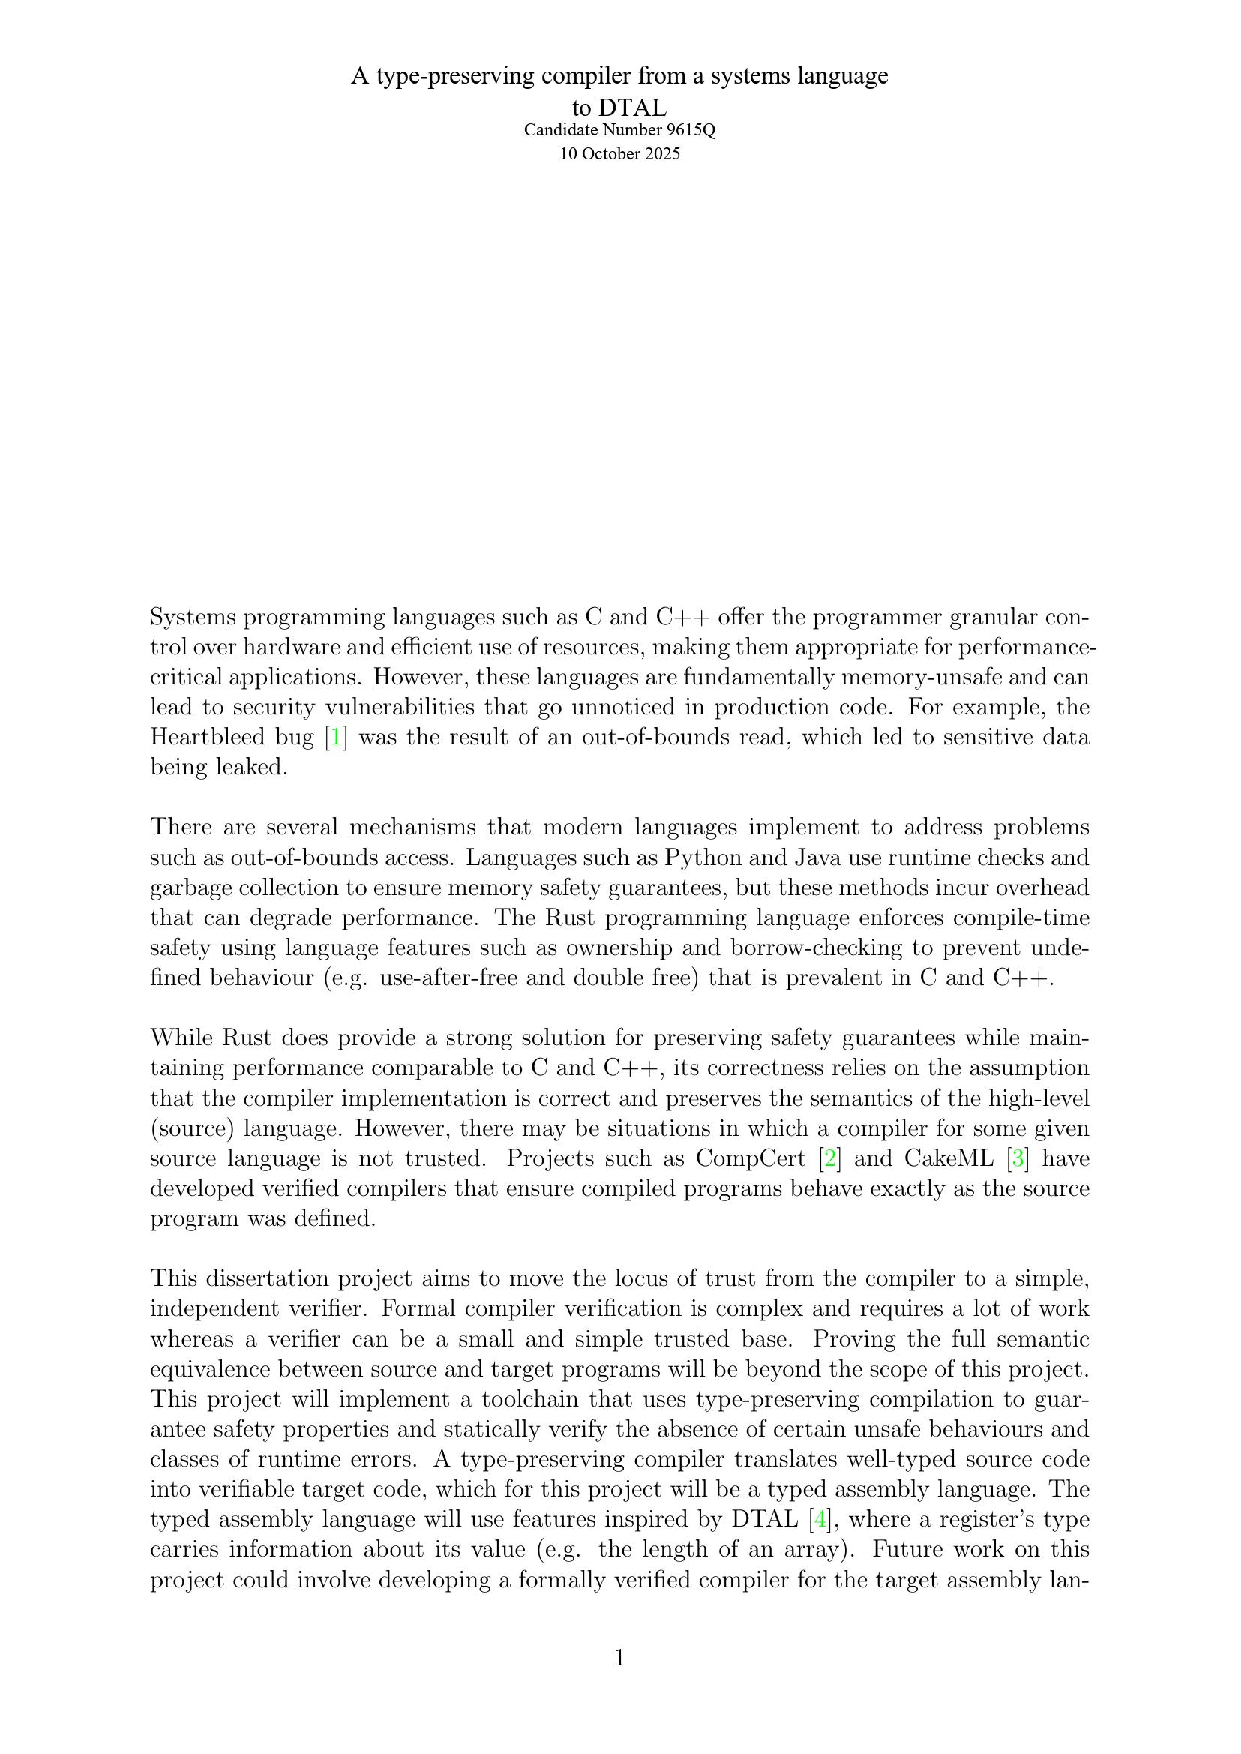
\includepdf[
  pages=1,
  pagecommand={\thispagestyle{empty}}
]{sources/proposal-page1-anonymised.pdf}

\includepdf[
  pages=2-,
  pagecommand={\thispagestyle{empty}}
]{sources/proposal.pdf}

%TC:endignore

\end{document}
